\documentclass[11pt,oneside]{book}

\usepackage[T1]{fontenc}
\usepackage[utf8]{inputenc}
\usepackage{lmodern}
\usepackage[margin=0.90in]{geometry}
\usepackage{amsmath,amssymb,mathtools}
\usepackage{proof}
\usepackage{listings}
\usepackage{xcolor}
\usepackage{booktabs,longtable,array,tabularx}
\usepackage{enumitem}
\usepackage{microtype}
\usepackage{tikz}
\usetikzlibrary{arrows.meta,positioning,fit,shapes.geometric,calc}
\usepackage{hyperref}

\hypersetup{
  colorlinks=true,
  linkcolor=blue!45!black,
  citecolor=green!35!black,
  urlcolor=magenta!45!black,
  pdftitle={From Inductive Definitions to a Checked Cyclic Certificate},
  pdfauthor={Cyclist Rocq project documentation}
}
\setcounter{tocdepth}{2}
\setcounter{secnumdepth}{3}
\setlength{\emergencystretch}{3em}
\renewcommand{\arraystretch}{1.14}
\linespread{1.04}

\definecolor{rocqblue}{RGB}{25,74,135}
\definecolor{rocqgreen}{RGB}{34,120,82}
\definecolor{rocqgray}{RGB}{95,99,104}
\definecolor{rocqback}{RGB}{247,248,250}
\lstdefinelanguage{Rocq}{
  morekeywords={From,Require,Import,Definition,Fixpoint,Inductive,Record,
    Module,Type,Parameter,End,Lemma,Theorem,Example,Proof,Qed,Defined,
    match,with,end,fun,forall,exists,let,in,if,then,else,return,as,
    destruct,intros,apply,exact,refine,unfold,rewrite,simpl,pose,set},
  sensitive=true,
  morecomment=[s]{(*}{*)},
  morestring=[b]"
}
\lstdefinestyle{rocq}{
  language=Rocq,
  basicstyle=\ttfamily\small,
  keywordstyle=\color{rocqblue}\bfseries,
  commentstyle=\color{rocqgreen},
  stringstyle=\color{magenta!60!black},
  numbers=left,
  numberstyle=\scriptsize\color{rocqgray},
  numbersep=8pt,
  frame=single,
  rulecolor=\color{black!18},
  backgroundcolor=\color{rocqback},
  breaklines=true,
  breakatwhitespace=false,
  columns=fullflexible,
  keepspaces=true,
  showstringspaces=false,
  tabsize=2,
  captionpos=b
}
\lstset{style=rocq}

\urlstyle{tt}
\DeclareRobustCommand{\code}[1]{\nolinkurl{#1}}
\DeclareRobustCommand{\file}[1]{\nolinkurl{#1}}
\newcommand{\src}[2]{\code{#2} in \file{#1}}
\newcommand{\Nat}{\mathbb{N}}
\newcommand{\sem}[1]{[\![#1]\!]}
\newcommand{\holds}{\models}
\newcommand{\notholds}{\not\models}
\newcommand{\Valid}{\mathsf{Valid}}
\newcommand{\rank}{\mathsf{rank}}
\newcommand{\FV}{\mathsf{F}}
\newcommand{\EV}{\mathsf{E}}
\newcommand{\mathintent}{\subsection*{Mathematical intention}}
\newcommand{\rocqreal}{\subsection*{Rocq realization}}
\newcommand{\soundlim}{\subsection*{Soundness and limitations}}
\newcommand{\takeaway}[1]{\begin{quote}\small\textbf{Reading invariant.} #1\end{quote}}
\newcommand{\rulebox}[1]{\fbox{\parbox{0.91\textwidth}{#1}}}

\title{\textbf{From Inductive Definitions to a Checked Cyclic Certificate}\\[0.7em]
  A Theory-to-Code Tutorial for \file{Rocq-copy/FirstOrder}}
\author{Cyclist Rocq project documentation}
\date{Source revision\\\code{08f6cd8834a3fc22088a064025abb9ee65c7f545}}

\begin{document}
\hypersetup{pageanchor=false}
\frontmatter
\maketitle
\hypersetup{pageanchor=true}

\chapter*{Purpose and reader contract}
\addcontentsline{toc}{chapter}{Purpose and reader contract}

This tutorial is for a reader who already knows first-order logic, inductive
definitions, and advanced Rocq.  Its question is not merely how the program
searches, but what theorem a successful computation produces.  The answer is
followed from the object language through ranked semantics, theorem-backed
rules, a finite cyclic graph, executable checks, a dependent certificate, and
finally semantic validity.

The exposition is tied to source revision
\code{08f6cd8834a3fc22088a064025abb9ee65c7f545}.  The eleven
\file{FirstOrder/*.v} modules and the required portions of
\file{Cyclic/Relations.v} and \file{Cyclic/Framework.v} are covered.  Historical
plans and the implementation audit help locate design decisions, but the
checked source is authoritative.

Three phrases are used precisely:
\begin{description}[leftmargin=3.2cm,style=nextline]
\item[semantic validity] a proposition quantified over every interpretation
and valuation, not a Boolean test;
\item[certified proof] a graph and finite witness packaged with the semantic
fields required by the generic soundness theorem;
\item[bounded non-success] a search returned \code{None} within a finite bound,
which is neither invalidity nor a countermodel.
\end{description}

Every code excerpt is introduced by the mathematical object it realizes.
Every operational success is connected to a checked theorem.  Every known gap
is stated as a completeness or interface limitation, never blurred into a
soundness qualification.

\tableofcontents

\mainmatter

\chapter{Orientation: the theorem-producing path}
\label{ch:orientation}

\mathintent

An automated prover should return evidence whose acceptance entails truth.
The architecture studied here factors that evidence into six stages:
\[
 \boxed{\text{judgment}}
 \longrightarrow \boxed{\text{rule generation}}
 \longrightarrow \boxed{\text{proof graph}}
 \longrightarrow \boxed{\text{checks}}
 \longrightarrow \boxed{\text{certificate}}
 \longrightarrow \boxed{\text{semantic validity}}.
\]
A judgment is finite syntax.  A generator chooses only rules that already
contain semantic proofs.  Search arranges such instances into a finite graph.
Boolean checks validate graph shape and global trace information.  Reflection
converts successful Booleans into dependent evidence.  A well-founded descent
then excludes a root countermodel.  This object-logic/generic-engine split is
the main architectural idea behind Cyclist \cite{brotherston2012generic}.

\rocqreal

Figure~\ref{fig:dependency-map} shows the source-level route.  Solid arrows are
logical or executable dependencies relevant to a theorem-producing run;
dashed arrows are concrete libraries and clients.  All eleven FirstOrder
modules appear.

\begin{figure}[p]
\centering
\resizebox{\textwidth}{!}{%
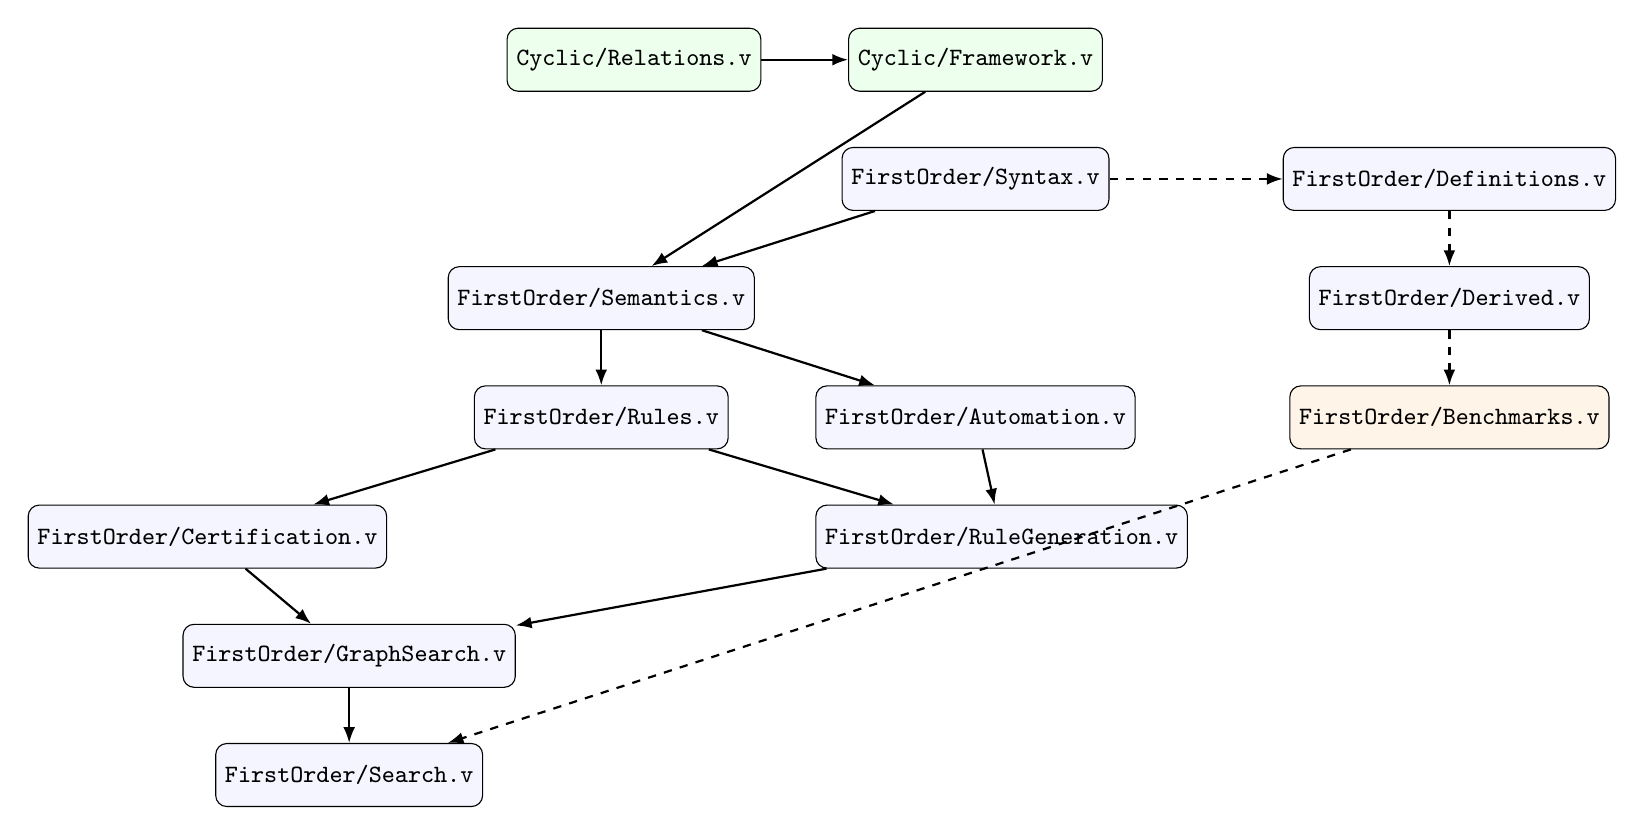
\begin{tikzpicture}[
  node distance=7mm and 11mm,
  box/.style={draw,rounded corners,align=center,minimum width=31mm,
              minimum height=8mm,fill=blue!4,font=\small\ttfamily},
  cbox/.style={box,fill=green!7},
  client/.style={box,fill=orange!9},
  arr/.style={-{Latex[length=2mm]},thick},
  darr/.style={arr,dashed}
]
\node[cbox] (rel) {Cyclic/Relations.v};
\node[cbox,right=of rel] (fw) {Cyclic/Framework.v};
\node[box,below=of fw] (syn) {FirstOrder/Syntax.v};
\node[box,below left=of syn] (sem) {FirstOrder/Semantics.v};
\node[box,below=of sem] (rules) {FirstOrder/Rules.v};
\node[box,right=of rules] (auto) {FirstOrder/Automation.v};
\node[box,below left=of rules] (cert) {FirstOrder/Certification.v};
\node[box,below right=of rules] (gen) {FirstOrder/RuleGeneration.v};
\node[box,below=of cert,xshift=18mm] (graph) {FirstOrder/GraphSearch.v};
\node[box,right=of syn,xshift=11mm] (defs) {FirstOrder/Definitions.v};
\node[box,below=of defs] (derived) {FirstOrder/Derived.v};
\node[client,below=of derived] (bench) {FirstOrder/Benchmarks.v};
\node[box,below=of graph] (search) {FirstOrder/Search.v};

\draw[arr] (rel) -- (fw);
\draw[arr] (fw) -- (sem);
\draw[arr] (syn) -- (sem);
\draw[arr] (sem) -- (rules);
\draw[arr] (sem) -- (auto);
\draw[arr] (rules) -- (cert);
\draw[arr] (rules) -- (gen);
\draw[arr] (auto) -- (gen);
\draw[arr] (cert) -- (graph);
\draw[arr] (gen) -- (graph);
\draw[arr] (graph) -- (search);
\draw[darr] (syn) -- (defs);
\draw[darr] (defs) -- (derived);
\draw[darr] (derived) -- (bench);
\draw[darr] (bench) -- (search);
\end{tikzpicture}
}
\caption{Complete module map for the documented FirstOrder implementation and
the required generic Cyclic substrate.}
\label{fig:dependency-map}
\end{figure}

At the public boundary, \src{FirstOrder/Search.v}{search_sound} is exactly the
one-way contract
\begin{equation}
  \mathsf{solvedb}(c,J)=\mathsf{true}
  \quad\Longrightarrow\quad
  \Valid(J).
  \label{eq:public-contract}
\end{equation}
The right side abbreviates \(\forall w,\sem{J}(w)\).  It does not say that
every valid \(J\) is found, and it does not turn \code{false} into a refutation.

\soundlim

The trust-bearing direction is from checked evidence to semantics.  Bugs in
candidate order or DFS can lose proofs; they cannot manufacture a theorem
unless they also pass the graph checks and the proof fields stored in each rule
record.  There is, however, an important operational qualification: the public
strategy currently tries general graph search and then exact theorem-backed
benchmark fallbacks.  Thus the nine public \code{true} results are certified,
but they are not nine demonstrations that general DFS alone rediscovered the
proofs.  Chapters~\ref{ch:graph-search} and~\ref{ch:bench-search} keep that
distinction explicit.

\chapter{The mathematical object language}
\label{ch:object-language}

\mathintent

Before reading \file{Syntax.v}, fix two disjoint, countable classes of
variables:
\[
  \mathcal V = \{\FV_0,\FV_1,\ldots\}
       \uplus \{\EV_0,\EV_1,\ldots\}.
\]
Free variables obtain values from the world being tested.  Existential
variables are interpreted only on the right of a sequent, by a witness
valuation.  Terms form a free algebra
\[
 t ::= c_n \mid x \mid f(t_1,\ldots,t_k),
\]
with natural-number constants and string-named function symbols.  In the
concrete library \(0\) is \(c_0\), \(s(t)\) is a unary function tree, and
\(\mathsf{cons}(h,t)\) is binary.

Atoms are
\[
 t=u,\qquad t\ne u,\qquad P^{\tau}(t_1,\ldots,t_k),
\]
where \(\tau\in\Nat\) is an optional trace tag.  Tags affect cyclic tracing,
not atom truth.  A product is a conjunction \(a_1\land\cdots\land a_m\); a
formula is a disjunction of products.  Therefore a formula is in disjunctive
normal form by construction.  The empty product is truth and the empty formula
is falsehood.

A sequent is \(L\vdash R\), where both sides are DNF formulae.  A judgment
also stores an ordered definition environment.  Each definition clause is a
Horn-style production
\[
  B_1\land\cdots\land B_m \Longrightarrow P(t_1,\ldots,t_k),
\]
represented by a body product and a head term list; the predicate name comes
from the environment lookup.  Substitutions are finite, first-match association
lists from variables to terms.

Freshness serves two independent purposes.  A fresh variable offset prevents
clause-local identifiers from capturing goal identifiers during unfolding.  A
fresh trace tag distinguishes the recursive predicate occurrences produced by
a left unfold.  Tag preparation supplies tags to previously untagged
antecedent predicates while preserving tags already present.

\rocqreal

The core declarations in \file{FirstOrder/Syntax.v} closely follow those
mathematical layers:
\begin{lstlisting}[caption={The reified object language; selected declarations from Syntax.v.}]
Inductive var_kind : Type := Free | Existential.
Record variable : Type := {
  variable_kind : var_kind;
  variable_id : nat
}.

Inductive term : Type :=
| Const (n : nat)
| Var (x : variable)
| Fun (name : string) (args : list term).

Inductive atom : Type :=
| Eq (left right : term)
| Neq (left right : term)
| Pred (tag : option nat) (name : string) (args : list term).

Definition product : Type := list atom.
Definition formula : Type := list product.
Record sequent : Type := { antecedent : formula; succedent : formula }.
Record clause : Type := { clause_body : product; clause_head : list term }.
Definition definitions : Type := list (string * list clause).
Record judgment : Type := {
  judgment_definitions : definitions;
  judgment_sequent : sequent
}.
\end{lstlisting}

The Boolean equalities are deliberately split.  \code{atom_eqb} is exact;
\code{atom_eqb_upto_tags} ignores only the optional tag on \code{Pred} and
keeps equation orientation exact.  This distinction is lifted through
products, formulae, sequents, and \src{FirstOrder/Syntax.v}{backlink_eqb}.
Ordinary graph labels use \code{judgment_eqb}; backlink comparison may ignore
tags because tags are proof annotations rather than logical content.

Substitution is a structurally recursive walk:
\begin{lstlisting}[caption={First-match substitutions and their action on terms.}]
Definition substitution : Type := list (variable * term).

Fixpoint lookup_substitution (s : substitution) (x : variable)
  : option term := ...

Fixpoint subst_term (s : substitution) (t : term) : term :=
  match t with
  | Const n => Const n
  | Var x => match lookup_substitution s x with
             | Some replacement => replacement | None => Var x end
  | Fun f xs => Fun f (map (subst_term s) xs)
  end.
\end{lstlisting}
The operation is extended homomorphically to atoms, products, formulae, and
sequents.  The syntax module also supplies \code{shift_term}, which preserves
variable kind and increases identifiers, and \code{existential_shift_term},
which converts clause variables into fresh existential variables for right
unfolding.

Tags are collected by \code{product_tags}, \code{formula_tags}, and
\code{judgment_tags}.  The next tag is
\code{S (max_list (sequent_tags q))}.  The function \code{prepare_sequent}
threads a counter through the antecedent, attaching successive tags only to
untagged predicates.  It does not sort products, normalize formulas, or change
the right-hand side.

\soundlim

The syntax is intentionally reified and executable, but not a parser-level
surface language.  Constants are naturals, symbol arities are not enforced by
a global signature, variables carry numeric identifiers rather than user
names, and definition lookup uses the first matching string entry.  Products
and formulae are lists: their semantics is set-like, yet their syntax retains
order and duplicates until \file{Automation.v} normalizes them.  These choices
make computation and equality straightforward, but they explain why generators
must prove permutation-insensitive semantic facts and why exact backlinks are
more restrictive than logical equivalence.

\chapter{Ranked semantics for first-order judgments}
\label{ch:semantics}

\section{Constructor-tree values and valuations}

\mathintent

The intended domain is the Herbrand-style free constructor algebra.  Values
are finite trees, so distinct constants and distinct function heads never
collapse semantically.  A valuation \(\rho:\mathcal V\to\mathcal D\) evaluates
terms homomorphically:
\[
 \sem{c_n}_\rho=\mathsf{VConst}(n),\quad
 \sem{x}_\rho=\rho(x),\quad
 \sem{f(\vec t)}_\rho
   =\mathsf{VFun}(f,\sem{\vec t}_\rho).
\]
This free model validates constructor clash and congruence, and it validates
injectivity for every semantic \code{VFun}.  The rule generator nevertheless
uses left injectivity only for the source prover's explicit \code{s}/\code{cons}
whitelist.

\rocqreal

\begin{lstlisting}[caption={The semantic carrier and term evaluation in Semantics.v.}]
Inductive value : Type :=
| VConst (n : nat)
| VFun (name : string) (args : list value).

Definition valuation : Type := variable -> value.

Fixpoint eval_term (rho : valuation) (t : term) : value :=
  match t with
  | Const n => VConst n
  | Var x => rho x
  | Fun f xs => VFun f (map (eval_term rho) xs)
  end.
\end{lstlisting}
An \code{interpretation} contains one function
\code{predicate_rank : string -> list value -> option nat}.  Presence of a
natural witnesses predicate truth; the number is a derivation height.  Thus
\(P(\vec v)\) holds exactly when \(I(P,\vec v)=\mathsf{Some}(h)\) for some
\(h\).

\soundlim

The semantics is not parametric in an arbitrary first-order structure.  It
fixes a free constructor domain, and equality is equality of constructor trees.
This is stronger than uninterpreted first-order equality and is exactly what
justifies constant/function contradiction and constructor decomposition.  A
future quotient or equational theory would require re-proving those rules.

\section{Ranked inductive predicates}

\mathintent

An interpretation models a definition environment when it supports both
directions of clause reasoning:
\begin{enumerate}[leftmargin=*]
\item \emph{introduction}: a true clause body makes its head predicate true;
\item \emph{ranked inversion}: every ranked head instance comes from some
clause instance whose body is true, and each predicate in that body has a
strictly smaller rank.
\end{enumerate}
The first condition closes the relation under productions.  The second rules
out unsupported cycles such as defining \(P\) only from \(P\) at the same
height.  Equations and disequations in a body impose no rank condition because
they are not inductive calls.

\rocqreal

\begin{lstlisting}[caption={The two-sided model condition.}]
Definition body_decreases
    (i : interpretation) (rho : valuation) (p : product) (height : nat) : Prop :=
  forall tag name args,
    In (Pred tag name args) p ->
    exists child_height,
      i.(predicate_rank) name (eval_terms rho args) = Some child_height /\
      child_height < height.

Definition models (ds : definitions) (i : interpretation) : Prop :=
  (forall name c rho,
      In c (lookup_definition name ds) ->
      product_holds i rho c.(clause_body) ->
      predicate_holds i name (eval_terms rho c.(clause_head))) /\
  (forall name args height,
      i.(predicate_rank) name args = Some height ->
      exists c rho,
        In c (lookup_definition name ds) /\
        eval_terms rho c.(clause_head) = args /\
        product_holds i rho c.(clause_body) /\
        body_decreases i rho c.(clause_body) height).
\end{lstlisting}
The concrete introduction and inversion conveniences in
\file{FirstOrder/Derived.v}, \code{model_intro} and \code{model_elim}, are simply
the two projections of this conjunction, specialized to
\code{fo_definitions}.

\soundlim

The representation packages the rank into the interpretation rather than
constructing a least fixed point inside Rocq.  Sound rules rely only on the two
model obligations above.  The semantic class is therefore precisely the class
of ranked interpretations satisfying them; no unproved claim equating this
record with every possible external fixed-point presentation is needed.

\section{DNF truth and shared existential witnesses}

\mathintent

For an interpretation \(I\) and valuation \(\rho\), products and formulas mean
\[
 I,\rho\holds[a_1,\ldots,a_m]
   \iff \bigwedge_j I,\rho\holds a_j,
 \qquad
 I,\rho\holds[p_1,\ldots,p_n]
   \iff \bigvee_k I,\rho\holds p_k.
\]
The empty product is true and the empty formula false.  Right-hand
existentials use two valuations.  Define
\[
 (\rho\oplus\eta)(x)=
 \begin{cases}
 \rho(x),&x\text{ is free},\\
 \eta(x),&x\text{ is existential}.
 \end{cases}
\]
Then
\[
 \mathsf{right\_holds}(I,\rho,R)
   \iff \exists\eta.\ I,\rho\oplus\eta\holds R.
\]
The same \(\eta\) is used by every atom of the selected product.  This is the
essential point: witnesses are shared across a conjunction, but the disjunction
may choose any one product.

\rocqreal

\begin{lstlisting}[caption={Products, DNF formulae, and right-hand witnesses.}]
Fixpoint product_holds (i : interpretation) (rho : valuation)
    (p : product) : Prop :=
  match p with [] => True | a :: p' =>
    atom_holds i rho a /\ product_holds i rho p' end.

Definition formula_holds (i : interpretation) (rho : valuation)
    (f : formula) : Prop :=
  exists p, In p f /\ product_holds i rho p.

Definition merge_valuation (base witness : valuation) : valuation :=
  fun x => match x.(variable_kind) with
           | Free => base x | Existential => witness x end.

Definition right_holds (i : interpretation) (rho : valuation)
    (f : formula) : Prop :=
  exists witness, formula_holds i (merge_valuation rho witness) f.
\end{lstlisting}
A world is a pair \((I,\rho)\).  The sequent \(L\vdash R\) holds at that world
when \(I\) modeling the stored definitions and \(L\) holding under \(\rho\)
imply \code{right_holds} for \(R\).  A judgment denotes this implication, and
the generic \code{Cyclic.Valid} quantifies it over all worlds.

\soundlim

Because witnesses may differ from the base valuation on existential
variables, several apparently obvious structural steps need side conditions.
For example, an antecedent atom syntactically repeated on the right cannot be
discharged if it contains existential variables: it may be evaluated under two
different valuations.  Likewise splitting a right conjunction is currently
restricted to free formulae so independently obtained premise witnesses can be
combined safely.

\section{Trace ranks}

\mathintent

A trace follows tagged inductive atoms in the antecedent.  If tag \(t\) marks
a true predicate whose stored derivation height is \(h\), its semantic rank is
\(h+1\).  If the tagged predicate is false, its rank is zero.  Missing tags also
have total rank zero.  The added one reserves zero as a useful false/missing
sentinel and makes strict progress on a true unfolded call visible.

\rocqreal

\src{FirstOrder/Semantics.v}{rank_atom} compares tags, consults
\code{predicate_rank}, and returns \code{Some (S height)} or \code{Some 0}.
\code{rank_product} and \code{rank_formula} scan left to right; hence duplicate
tags would make position matter.  Left-unfold generation prevents a selected
tag from appearing in the skipped prefix, while \code{prepare_sequent} normally
gives distinct tags.  \code{rank_of_tag} reads only the antecedent.  The module
\code{FirstOrderTheory} then instantiates the generic interface with worlds,
judgments, exact and backlink equality, denotation, tag collection, and rank.

\soundlim

Tags do not change truth, but they do change trace routing.  Tag-insensitive
backlink equality is therefore semantically sensible only because the backlink
rule separately supplies a checked edge relation.  Duplicate tags are not a
mere cosmetic issue: rank lookup chooses the first occurrence.  Generators
must maintain their stated uniqueness/position side conditions.

\chapter{The generic cyclic substrate}
\label{ch:cyclic}

\section{Local rules and countermodel propagation}

\mathintent

An ordinary sound rule says that validity of every premise entails validity of
the conclusion.  A cyclic proof needs more.  If the conclusion is false at a
world, the proof must be able to choose a false premise at a successor world
while respecting a relation between source and target trace tags.  For edge
information \(E=(V,P)\), the semantic obligation is
\[
 (a,b)\in V \Rightarrow \rank_b(w')\le\rank_a(w),\qquad
 (a,b)\in P \Rightarrow \rank_b(w')<\rank_a(w).
\]
Here \(P\subseteq V\) is checked structurally; \(V\) gives non-increase and
\(P\) strict progress.

\rocqreal

The central record in \file{Cyclic/Framework.v} makes both directions explicit:
\begin{lstlisting}[caption={A theorem-backed local cyclic rule.}]
Record rule_instance : Type := {
  rule_name : string;
  rule_conclusion : T.Judgment;
  rule_premises : list premise;
  rule_theorem : premises_valid rule_premises -> Valid rule_conclusion;
  rule_counter_step :
    forall w, ~ holds rule_conclusion w ->
    { k : nat & { p : premise & { w' : T.World |
      nth_error rule_premises k = Some p /\
      ~ holds p.(premise_judgment) w' /\
      respects_edge rule_conclusion p.(premise_judgment)
        w w' p.(premise_edge) } } }
}.
\end{lstlisting}
An \code{axiom_instance} is smaller: a label plus a proof of its validity.
FirstOrder rules build these records directly.  Search never installs a bare
string such as ``L.Unfold'' and asks the checker to trust its meaning.

\soundlim

\code{rule_theorem} alone would justify finite proof trees but not arbitrary
cycles.  \code{rule_counter_step} is the bridge from a hypothetical false root
to an infinite false path.  Conversely, a good countermodel transition without
the forward theorem would not be an acceptable user-facing inference.  Both
fields are part of every implemented rule.

\section{Finite graphs, backlinks, and structural checking}

\mathintent

A regular infinite derivation can be stored as a finite directed graph.  Each
node is open, closed by an axiom, expanded by a rule to fresh premise nodes, or
closed by a backlink to an existing companion.  A valid graph must have a root,
matching labels, in-bounds edges, well-formed trace pairs, correct rule arity,
no reflexive backlink, no open nodes, and no unreachable garbage.

\rocqreal

\code{node_kind} has constructors \code{OpenNode}, \code{AxiomNode},
\code{RuleNode}, and \code{BacklinkNode}.  The immutable operations
\code{graph_add_axiom}, \code{graph_apply_rule}, and
\code{graph_add_backlink} modify only an open node after Boolean equality and
bounds checks.  Rule application appends fresh open nodes; backlink application
requires a unary rule and uses both exact premise equality and the theory's
\code{backlink_eqb}.

The Boolean \src{Cyclic/Framework.v}{structural_check} verifies root equality,
all node payloads, edge well-formedness, and reachability from index zero.
Reachability is saturated for as many iterations as there are stored nodes.
This rejects a syntactically closed but disconnected collection of facts.

\soundlim

Graph closure is only a structural property.  A cycle of identity edges can be
closed and locally well formed yet fail the global progress condition.  Search
therefore distinguishes \code{graph_closedb} from a \code{checked_graph}; this
distinction is essential rather than administrative.

\section{Relations, closure, and infinite descent}

\mathintent

The size-change view abstracts each proof edge to arcs between trace tags,
labelled either \emph{stay} or \emph{decrease}.  Composition connects the
target tag of one arc to the source tag of the next.  If several routes produce
the same tag pair, decrease dominates stay.  A loop is acceptable only if the
transitive closure exposes a decreasing diagonal \((t,t)\).  This is the same
structural idea that turns local size comparisons into a global no-infinite-run
argument \cite{lee2001sizechange}, adapted here to proof traces.

\rocqreal

\file{Cyclic/Relations.v} defines \code{slope}, \code{arc}, relation union and
composition, bounded saturation by \code{relation_closure}, graph-path
relations, and \code{relational_trace_check}.  The algebra is tiny:
\[
 \mathsf{Decrease}\sqcup s=\mathsf{Decrease},\qquad
 \mathsf{Stay}\sqcup\mathsf{Stay}=\mathsf{Stay}.
\]
\code{path_closure} composes paths whose graph endpoints meet.
\code{loop_relation_ok} checks decreasing diagonals only when source and target
node indices agree.  In the framework, \code{relation_fuel} and
\code{graph_path_fuel} are finite bounds derived from graph tags and nodes.

\soundlim

The executable relational check is required by \code{raw_check}, but the
semantic certificate proof uses the more concrete finite witness described
next.  This is deliberate redundancy: passing the relation closure is an
additional acceptance condition, not the sole semantic witness consumed by
\code{certificate_sound}.  The tutorial does not identify the implementation
with every formulation of the global trace condition in the literature
\cite{brotherston2005cyclic,brotherston2011sequent}.

\section{Finite witnesses and lexicographic descent}

\mathintent

A finite trace witness assigns each node an optional selected tag and a natural
potential.  Before tag selection, every followed live edge must decrease the
potential.  The witness may switch once from no tag to some tag.  After
selection, it cannot drop the tag; it follows a valid pair, and each step either
has semantic progress or decreases the auxiliary potential.  This turns the
qualitative assertion ``some trace progresses infinitely often'' into a local,
finite routing object.

\rocqreal

\begin{lstlisting}[caption={Finite trace-routing data and its transition relation.}]
Record trace_witness : Type := {
  witness_tag : nat -> option nat;
  witness_potential : nat -> nat
}.

Definition trace_transition (tw : trace_witness)
    (i j : nat) (e : edge_info) : Prop :=
  match tw.(witness_tag) i, tw.(witness_tag) j with
  | None, None => tw.(witness_potential) j < tw.(witness_potential) i
  | None, Some _ => True
  | Some _, None => False
  | Some a, Some b =>
      In (a,b) e.(edge_valid) /\
      (In (a,b) e.(edge_progress) \/
       tw.(witness_potential) j < tw.(witness_potential) i)
  end.
\end{lstlisting}
Only edges whose target is \emph{live} are constrained.  Here
\code{liveb g i} means a path of length equal to the number of graph nodes
starts at \(i\); in a finite graph such a path reaches a cycle.  The complete
Boolean acceptance test is
\[
 \mathsf{raw\_check}(G,W)=
 \mathsf{structural\_check}(G)\land
 \mathsf{relational\_check}(G)\land
 \mathsf{witness\_check}(G,W).
\]

The certificate adds non-Boolean semantic fields: root existence and equality,
false-node liveness, a false-successor/countermodel step, and propositional
trace transitions.  Its descent measure has two phases:
\[
 \mathsf{BeforeTrace}(p)\mapsto(1,(p,0)),\qquad
 \mathsf{FollowingTrace}(r,p)\mapsto(0,(r,p)).
\]
Nested lexicographic order over naturals is well founded.  Selecting a trace
decreases the leading component; later steps decrease semantic rank or, when
rank merely stays, the finite potential.  The theorem
\src{Cyclic/Framework.v}{certificate_step_decreases} constructs a smaller
false successor.  \src{Cyclic/Framework.v}{certificate_sound} assumes a false
root and iterates that step by well-founded induction, producing a
contradiction.

\soundlim

The theorem uses classical double-negation elimination and the framework's
constructive-choice machinery elsewhere in the development contributes to the
reported assumptions of the public search theorem.  These are logical-library
assumptions printed by Rocq, not unchecked application axioms.  Exact outputs
are recorded in Chapter~\ref{ch:trust}.

\chapter{The implemented inference rules I: logical structure}
\label{ch:rules-logic}

The recurring implementation pattern is worth fixing.  First write a sequent
rule.  Then identify how a false conclusion chooses a false premise and which
tag pairs are non-increasing or progressing.  Only then package both proofs in
a \code{Cyclic.rule_instance}.  This order prevents an executable generator
from becoming the specification.

\section{Identity modulo tags and ex falso}

\mathintent

Identity closes a singleton antecedent when some right product is contained in
the antecedent product, comparing predicate atoms modulo tags:
\[
 \infer[\mathrm{Id}/\tau]
       {A\vdash R_0\lor B\lor R_1}
       {B\subseteq_{\tau}A}
\]
The line above is an axiom schema: the displayed condition is checked by the
generator, not a proof premise.  The selected product must be free so the base
valuation itself supplies the right witness.  Equality and disequality remain
oriented and exact.

Ex falso recognizes either a reflexive disequality or a constructor clash:
\[
 \infer[\bot_L]{A,(t\ne t),A'\vdash R}{ }
 \qquad
 \infer[\mathsf{clash}_L]
       {A,(c_n=f(\vec t)),A'\vdash R}{ }.
\]
The symmetric function/constant orientation is also implemented.

\rocqreal

\src{FirstOrder/Rules.v}{identity_axiom_anywhere_upto_tags} is named
\code{"Id/modulo-tags"}.  It accepts any RHS product position and a semantic
subset proof obtained from \code{product_subsetb_upto_tags_spec}.
\code{disequality_axiom} and \code{constructor_clash_axiom_left/right} are
named \code{"Ex Falso"}.  In \file{RuleGeneration.v},
\code{identity_candidate} scans right products, while
\code{contradiction_candidate} scans the unique antecedent product.

\soundlim

The generator requires a singleton antecedent.  A disjunctive antecedent must
first be split.  Constructor clash is broader than the old zero-versus-specific
constructor test because the semantic domain makes every constant distinct
from every function tree.  Identity ignores predicate tags only; it does not
commute equality arguments or rearrange term lists.

\section{Left disjunction and restricted right conjunction}

\mathintent

With DNF lists, left disjunction chooses which product makes the antecedent
true.  The binary decomposition is
\[
 \infer[L.\lor]
       {p\lor P\vdash R}
       {p\vdash R & P\vdash R}.
\]
Repeated use enumerates every antecedent product.  A single right product is a
conjunction, so the implemented right rule splits its head atom from the rest:
\[
 \infer[R.\land]
       {L\vdash a\land B}
       {L\vdash a & L\vdash B}.
\]
The logical rule needs compatible existential witnesses.  The current kernel
uses the sufficient condition that the antecedent and both right pieces are
free; then witness values are irrelevant and the two premise proofs combine.

\rocqreal

\code{left_disjunction_rule} contains two premise records with empty trace
edges, because no tagged inductive atom is being related across its split.
Its countermodel proof inspects the product chosen by
\code{formula_holds}.  \code{right_conjunction_rule} uses identity edges and
the lemmas \code{right_holds_free} and \code{product_holds_merge_free}.
Generators \code{left_disjunction_candidate} and
\code{right_conjunction_candidate} recognize the exact list shapes.

\soundlim

The right rule is intentionally narrower than the mathematically strongest
DNF conjunction rule.  Independent witnesses could also be combined when the
existential-variable sets of the pieces are pairwise disjoint; that condition
is not implemented.  Search failure on such a goal is incompleteness, not a
problem with \code{search_sound}.

\section{Reflexive equality elimination}

\mathintent

Reflexive equality is semantically true, so it may be removed from either side:
\[
 \infer[\mathsf{Simpl}{=}L]
       {A,(t=t),A'\vdash R}{A,A'\vdash R}
 \qquad
 \infer[\mathsf{Simpl}{=}R]
       {L\vdash R_0\lor(B\land t=t\land B')\lor R_1}
       {L\vdash R_0\lor(B\land B')\lor R_1}.
\]
Removing an equality does not alter a predicate trace rank.

\rocqreal

\code{reflexive_equality_rule} proves both semantic equivalence and rank
equality, then invokes the reusable \code{equivalence_rule}.  The arbitrary
right-position wrapper is \code{right_reflexive_equality_rule}.  Their
generators remove exactly one selected equality; the next graph node repeats
simplification if needed.  The records are named \code{"Simpl ="}.

\soundlim

The implementation does not filter every reflexive equality in one graph
step.  This changes graph size and fuel consumption but not the logical result
of repeated applications.  Left scanning remains limited to a singleton
antecedent, whereas right scanning visits every product and atom.

\chapter{The implemented inference rules II: equality and structure}
\label{ch:rules-equality}

\section{Left equality substitution}

\mathintent

If a free variable is equated to a free term, replace it throughout the
remaining sequent:
\[
 \infer[\mathsf{EqSubst}]
       {A,(x=t),A'\vdash R}
       {A[x:=t],A'[x:=t]\vdash R[x:=t]}
 \quad
 \begin{array}{l}
 x\text{ free},\ t\text{ free},\\[-0.2em]
 x\notin t\text{ by the checked shape used here.}
 \end{array}
\]
At a world satisfying \(x=t\), evaluating any substituted term agrees with
evaluating the original.  Therefore truth and trace ranks transport.

\rocqreal

\src{FirstOrder/Rules.v}{left_equality_substitution_rule} stores the rule name
\code{"Eq subst"}.  Its proof is built from structural lemmas
\code{eval_term_single_subst_equal},
\code{atom_holds_single_subst_equal}, and their product/formula/rank lifts.
\code{find_left_equality_substitution} recognizes only a free variable
syntactically on the left of an equation and a free replacement.

\soundlim

The reverse orientation \(t=x\) is not connected on the left, even though
some cases are sound.  Nor is the rule a general equality solver.  The narrow
shape makes its valuation proof direct and avoids hidden cyclic substitutions.

\section{Right existential solving and orientation}

\mathintent

Inside one selected right product, an equation can assign a witness variable:
\[
 \infer[\exists\mathsf{Solve}]
       {L\vdash R_0\lor(B\land \EV_x=t\land B')\lor R_1}
       {L\vdash R_0\lor(B[\EV_x:=t]\land B'[\EV_x:=t])\lor R_1}
 \quad t\text{ free}.
\]
The conclusion witness is obtained from the premise witness by overriding
\(\EV_x\) with the base interpretation of \(t\).  The symmetric equation
\(t=\EV_x\) is first oriented.

\rocqreal

\code{single_existential_substitution} and
\code{existential_solution_valuation} formalize that override.
\code{right_existential_substitution_rule} is named
\code{"Eq existential/right"}; its arbitrary-position wrapper preserves other
products.  \code{right_equality_orientation_rule} swaps only the selected
equation.  The simplifier tries direct solving, then orientation, and on the
next node solves the oriented result.

\soundlim

This is right-side witness solving, not the missing whole-sequent
\emph{existential instantiation} rule of the original prover.  It requires a
free replacement and does not solve existential-to-existential cycles or
arbitrary terms containing existential variables.

\section{Right discharge}

\mathintent

An atom already supplied by a singleton antecedent may be removed from a right
product:
\[
 \infer[\mathsf{Discharge}_R]
       {a,A\vdash R_0\lor(B\land a\land B')\lor R_1}
       {a,A\vdash R_0\lor(B\land B')\lor R_1}.
\]
Predicate comparison ignores tags, because tags do not affect truth.  The
discharged atom must be free so its truth under the base valuation persists
under the merged right witness.

\rocqreal

\code{right_discharge_rule} uses
\code{atom_eqb_upto_tags_holds} and \code{atom_holds_merge_free};
\code{right_discharge_candidate} searches every right product and position.
The rule is generated before constructor equality decompositions, matching the
documented simplifier priority.

\soundlim

Dropping the free-atom check would be unsound: an existential variable in the
antecedent is read from \(\rho\), but the same syntax on the right is read from
\(\rho\oplus\eta\).  The regression
\code{generated_right_discharge_rejects_existential_atom} fixes this boundary.

\section{Constructor-equality decomposition}

\mathintent

On the right, congruence reduces equality of same-headed, equal-arity function
terms to component equations:
\[
 \infer[\mathsf{FunEq}_R]
       {L\vdash R_0\lor(B\land f(\vec s)=f(\vec t)\land B')\lor R_1}
       {L\vdash R_0\lor(B\land \bigwedge_i s_i=t_i\land B')\lor R_1}.
\]
In a free constructor algebra the converse is also valid.  The left rule uses
that injectivity, but only for the configured constructors \(s\) and
\(\mathsf{cons}\):
\[
 \infer[\mathsf{Inj}_L]
       {A,f(\vec s)=f(\vec t),A'\vdash R}
       {A,(s_1=t_1),\ldots,(s_k=t_k),A'\vdash R}.
\]

\rocqreal

\code{equation_product} zips equal-length argument lists.  The semantic and
rank lemmas justify \code{right_function_equality_rule} and
\code{left_function_equality_rule}.  \code{injective_constructorb} accepts
only the strings \code{"s"} and \code{"cons"}.  Both generators scan arbitrary
positions and reject arity mismatch safely.

\soundlim

Right decomposition needs only congruence and therefore accepts any matching
function name.  Left decomposition uses injectivity and intentionally follows
the source prover's whitelist, despite the local semantic domain validating
more constructors.  Generalizing the whitelist is sound for the current
semantics but would be an interface and search-policy change, not a mere proof
cleanup.

\chapter{The implemented inference rules III: cyclic structure}
\label{ch:rules-cyclic}

\section{Explicit weakening and free substitution}

\mathintent

Non-exact backlinks are prepared by ordinary proof steps rather than hidden
inside the backlink checker.  Prefix weakening removes extra antecedent atoms:
\[
 \infer[\mathsf{Weak}]
       {A,E\vdash R}
       {A\vdash R}.
\]
Free substitution moves from a general companion to its instance:
\[
 \infer[\mathsf{Subst}]
       {\sigma(L)\vdash\sigma(R)}
       {L\vdash R},
 \qquad \sigma\text{ maps only free variables to free terms}.
\]
These directions are chosen so that the current open node becomes exactly the
ancestor label after one or more explicit steps.

\rocqreal

\code{prefix_weakening_rule} is named \code{"Weaken"} and retains rank
information for tags in the smaller prefix.  \code{free_substitutionb} checks
both domain kinds and range terms.  The general rule
\code{general_free_substitution_rule}, named \code{"Subst"}, constructs a new
valuation by evaluating substituted terms and proves truth/rank transport.
\file{GraphSearch.v} invokes these records while preparing backlinks.

\soundlim

Weakening is prefix-only, not arbitrary set subsumption.  Judgment matching
flattens terms, directionally matches them, and then rechecks the entire
substituted judgment exactly.  This is a sound but narrow substitute for full
formula/product unification and subsumption.

\section{Matched and equation-producing right unfolding}

\mathintent

Suppose \(P(\vec h)\leftarrow B\) is a definition clause and a directional
match \(\sigma(\vec h)=\vec t\) succeeds.  Right introduction replaces the
selected goal predicate by the instantiated clause body:
\[
 \infer[R.\mathsf{Unfold}/\mathsf{match}]
       {L\vdash R_0\lor(A\land P(\vec t)\land A')\lor R_1}
       {L\vdash R_0\lor(A\land \sigma(B)\land A')\lor R_1}.
\]
When matching fails but arities agree, the fallback shifts clause variables to
fresh right existential variables and emits head equations:
\[
 \infer[R.\mathsf{Unfold}]
       {L\vdash R_0\lor(A\land P(\vec t)\land A')\lor R_1}
       {L\vdash R_0\lor
        (A\land B^{\exists}\land\vec t=\vec h^{\exists}\land A')\lor R_1}.
\]
Clause introduction proves both rules: satisfying the body under a clause
valuation makes the head predicate true.

\rocqreal

\code{matched_right_unfold_rule} and its arbitrary-position wrapper carry a
proof from \code{match_terms_sound}; their name is
\code{"R.Unfold/match"}.  \code{right_unfold_rule} and
\code{standard_right_unfold_at_rule} implement the equation-producing
fallback, named \code{"R.Unfold"}.  The latter uses
\code{existential_shift_product} and \code{equation_product}.  Both preserve
the left trace ranks with identity-style edges.

\soundlim

Directional matching binds pattern variables only.  The standalone symmetric
unifier is not integrated into right unfolding, so the behavior is not the
source prover's full multi-unification with residual equations.  Matched
unfolding is tried before left unfolding; the equation-producing family is
placed after left unfolding to avoid spending DFS fuel prematurely on weak
constraint branches.

\section{Ranked left unfolding}

\mathintent

Left unfolding is the induction-bearing rule.  For a tagged antecedent atom
\(P^t(\vec u)\), ranked inversion chooses one defining clause.  To prove the
conclusion, every possible clause must be handled:
\[
 \infer[L.\mathsf{Unfold}]
       {A,P^t(\vec u),A'\vdash R}
       {\{\ A,B_c^{\uparrow,t_c},\vec u=\vec h_c^{\uparrow},
                 P^t(\vec u),A'\vdash R\ \}_{c\in\mathsf{def}(P)}}.
\]
The schematic premise retains the selected predicate as a contraction point.
Clause variables are freshly shifted.  Body predicates receive a fresh tag.
An edge relates the source tag to both contraction and body tags; recursive
body occurrences carry strict progress because ranked inversion makes their
heights smaller.

\rocqreal

\code{left_unfold_product}, \code{left_unfold_judgment}, and
\code{left_unfold_premises} construct the branches.  The proof
\code{left_unfold_respects} uses model inversion to select the false premise
and establish edge inequalities.  \code{left_unfold_rule}, named
\code{"L.Unfold"}, produces one premise per clause.  The
arbitrary-position wrapper \code{left_unfold_at_rule} rotates products while
proving truth and rank invariance.

The generator requires a singleton antecedent, a selected tagged predicate, a
fresh distinct tag, variable-bound checks, a free RHS, and no duplicate
selected tag in the skipped prefix.  It scans every atom of the unique product
in source order.

\soundlim

The free-RHS restriction means left unfolding is not connected when the right
side contains existential variables.  There is no dedicated composed
left-unfold-then-right-unfold candidate.  Both choices reduce search coverage,
not rule soundness.  The contraction copy is crucial: it provides the repeated
shape against which a later backlink can close.

\section{Exact backlinks}

\mathintent

A backlink identifies a repeated sequent after ordinary preparation steps:
\[
 \infer[\mathsf{Backlink}]{J}{J}.
\]
This rule is locally just semantic equivalence.  Its cyclic force comes from
where its only premise points in the finite graph and from progress accumulated
along the complete loop.  The backlink edge itself preserves each antecedent
tag; it need not be the edge on which strict decrease occurred.

\rocqreal

\code{exact_backlink_rule} specializes \code{backlink_rule} to the same
judgment with \code{identity_edge}.  Search considers every earlier node index.
\code{graph_add_backlink} independently checks source conclusion, target
premise, tag-insensitive backlink equality, bounds, unary arity, and
non-reflexivity.

\soundlim

The final backlink is exact in list shape and logical syntax.  Tag-insensitive
comparison alone is not a general subsumption algorithm.  Substitution and
prefix weakening can prepare some companions, but arbitrary reordering,
set-based weakening, equation orientation alternatives, and selected-tag
minimization are absent.  Folding before backlinking is entirely absent.

\chapter{Verified executable infrastructure}
\label{ch:automation}

\file{FirstOrder/Automation.v} is not a bag of trusted tactics.  It defines
total Gallina programs, proves small reflection or preservation lemmas around
their results, and lets later modules consume only those proved interfaces.
This chapter follows its three main layers: set-style normalization, variable
analysis, and term solving.

\section{Normalization and Boolean reflection}

\mathintent

Although products and formulae are stored as lists, conjunction and disjunction
are idempotent and insensitive to duplicates.  A safe normalization may remove
duplicates without changing denotation:
\[
 \sem{\mathsf{nodup}(p)}=\sem p,
 \qquad
 \sem{\mathsf{nodup}(\mathsf{map}\;\mathsf{nodup}\;F)}=\sem F.
\]
No sorting is mathematically required for this fact.  Exact Boolean equality
can then serve as a decidable guard, provided a reflection theorem connects
\code{eqb = true} to propositional equality.

\rocqreal

\code{normalize_product} is \code{nodup atom_eq_dec};
\code{normalize_formula} maps product normalization and removes duplicate
products.  The chain
\code{normalize_product_holds}, \code{normalize_formula_holds},
\code{normalize_right_holds}, \code{normalize_sequent_holds}, and
\code{normalize_judgment_valid} proves preservation at every layer.  This last
equivalence is why a public \code{verified_proof} may certify the normalized
root and still yield validity of the exact input.

Set-like Boolean helpers have specifications rather than being assumed:
\code{product_set_eqb_spec} characterizes mutual membership, and
\code{product_mem_setb_spec} characterizes membership of a product modulo atom
permutation.  The syntax module similarly provides \code{term_eqb_spec},
\code{atom_eqb_spec}, \code{product_subsetb_spec}, and the tag-insensitive
subset specification.

\soundlim

Normalization removes duplicates but does not canonicalize order.  Two
logically equivalent permutations can therefore remain syntactically unequal.
Later exact checks deliberately remain conservative.  Replacing \code{nodup}
with a canonical ordering would require an ordering on all reified syntax and
new preservation/equality results.

\section{Variables and freshness}

\mathintent

Matching and unfolding need explicit finite variable information: variables
occurring in a term, whether a variable belongs to the free or existential
class, and identifiers unused by an entire sequent.  Freshness is numerical:
one plus the maximum identifier suffices because syntax is finite.

\rocqreal

\code{term_variables} recursively concatenates variables from function
arguments.  Atom, product, formula, and sequent collectors lift it.
\code{is_free_variable} and \code{is_existential_variable} inspect
\code{variable_kind}; \code{fresh_free_variable} and
\code{fresh_existential_variable} reuse \code{fresh_variable_offset} with the
desired kind.  \code{term_is_existential_variable} recognizes the exact
single-variable term shape used by right equality solving.

\soundlim

These collectors are executable analyses, not binders or a locally nameless
metatheory.  Capture avoidance is achieved by arithmetic shifting and checked
bounds.  Any extension that adds binders to terms would invalidate this simple
freshness story and require a new syntax and semantic substitution theory.

\section{Directional matching}

\mathintent

Directional matching treats the left list as patterns and the right list as
fixed targets.  It may bind a variable occurring in the pattern, but it does
not solve target variables symmetrically.  Repeated pattern variables must
receive consistent terms, constructors must have the same name and arity, and
the lists must have the same length.

The robust proof pattern is \emph{compute, then verify}:
\[
 \mathsf{rawMatch}(\vec p,\vec t)=\mathsf{Some}(\sigma),
 \quad
 \mathsf{eqb}(\sigma\vec p,\vec t)=\mathsf{true}
 \quad\Longrightarrow\quad
 \sigma\vec p=\vec t.
\]
Correctness of downstream rules depends on the final equality, not on a large
invariant about every branch of the heuristic algorithm.

\rocqreal

\code{zip_terms} creates an equation work list.  \code{match_equations} consumes
a structurally bounded amount of fuel, uses \code{add_match_binding} to reject
inconsistent rebinding, and descends through matching function heads.
\code{raw_match_terms} exposes that engine; \code{match_terms} re-applies the
candidate and checks \code{terms_eqb}.  The gate is:
\begin{lstlisting}[caption={The small theorem consumed by matched unfolding.}]
Lemma match_terms_sound patterns targets s :
  match_terms patterns targets = Some s ->
  map (subst_term s) patterns = targets.
\end{lstlisting}

\soundlim

Matcher fuel exhaustion is non-success.  Directionality is a design feature,
not a completeness theorem.  In particular, it does not reproduce the source
prover's multi-unification behavior for repeated variables and residual
equations.

\section{Substitution composition and symmetric unification}

\mathintent

Symmetric first-order unification may solve variables on either side.  When a
new binding \(x\mapsto t\) is found, it must update the remaining equations and
all old substitution ranges.  An occurs check rejects \(x\mapsto f(\ldots x
\ldots)\).  Composition order matters because association-list lookup uses the
first binding.

\rocqreal

\code{compose_substitution newer older} applies the newer substitution to old
ranges and then appends genuinely new-domain bindings.
\code{term_occursb} implements the structural occurs check.
\code{unify_equations} handles equality, variables in either orientation,
constant clash, and same-headed function decomposition.  A generous size-based
\code{unification_fuel} makes it total.  As with matching, the exported
\code{unify_terms} verifies the result by reapplying it to both sides, and
\code{unify_terms_sound} exposes only the proved equality.

Two source regressions record the intended behavior:
\begin{lstlisting}[caption={Executable unification boundaries.}]
Example unification_propagates_later_bindings :
  unify_terms [Var (free_var 0); Var (free_var 1)]
    [Var (free_var 1); Const 0] =
  Some [((free_var 1), Const 0); ((free_var 0), Const 0)].

Example unification_occurs_check :
  unify_terms [Var (free_var 0)]
    [succ (Var (free_var 0))] = None.
\end{lstlisting}

\soundlim

The unifier is verified when it succeeds, but the fuel bound is not proved
complete for all unifiable inputs.  More importantly, current rule generation
does not use it to implement general right unfolding or backlink subsumption.
It is verified infrastructure awaiting a carefully specified integration.

\chapter{From syntax to candidate rules}
\label{ch:generation}

\section{Priority is operational semantics}

\mathintent

A rule kernel describes what an inference means.  A generator describes where
to apply it and in what order alternatives should be explored.  The distinction
is important: two generators can be equally sound but have very different
coverage and runtime.  Candidate order is therefore part of the executable
behavior, even though it is not part of the validity theorem.

\rocqreal

\file{FirstOrder/RuleGeneration.v} first tries an axiom.  Within
\code{generate_axiom}, identity is tried before contradiction.  The single
\code{simplification_candidate} returns at most one rule, in this precise
order for singleton antecedents:
\begin{enumerate}[leftmargin=*]
\item left reflexive equality;
\item right reflexive equality;
\item left equality substitution;
\item right existential solving or orientation;
\item right discharge;
\item left constructor injectivity;
\item right function congruence.
\end{enumerate}
With a non-singleton antecedent, left-only simplifications and discharge are
unavailable; right reflexivity, existential solving, and function equality
remain.

The ordinary list returned by \code{generate_rules} is ordered as
\[
 L.\lor, R.\land, R.\mathsf{Unfold}/\mathsf{match},\
 L.\mathsf{Unfold},\ R.\mathsf{Unfold}\text{ with equations}.
\]
Every item is already a complete \code{rule_instance}; the generator does not
emit unverified descriptors.

\soundlim

This order mirrors only the implemented portion of the source prover.  There
is no folding family, no general existential instantiation, and no composed
left/right unfold primitive.  Moving a sound candidate earlier cannot make the
system unsound, but it can make bounded DFS miss proofs it previously found by
using the bound on a worse branch.

\section{Scanning arbitrary positions}

\mathintent

List representation should not restrict a set-like logical rule to the first
atom.  A standard technique carries a prefix accumulator \(B\), inspects the
head \(a\) of the remaining list, and reconstructs the source as
\(B\mathbin{++}a::A\).  For nested DNF, one accumulator tracks prior products
and another prior atoms.  A transport lemma proves that rotating or replacing
at the chosen position preserves semantics and the relevant ranks.

\rocqreal

This pattern appears in \code{find_right_reflexive_in_product/formula},
\code{find_right_existential_in_product/formula},
\code{find_right_discharge_in_product/formula}, both function-equality scans,
and right unfolding.  Left unfolding scans every atom of the unique
antecedent product and uses \code{left_unfold_at_candidate} to establish the
no-duplicate-tag side condition before constructing a wrapper record.

\soundlim

Arbitrary position does not mean arbitrary logical equivalence.  Prefix
accumulators preserve the exact order of untouched atoms and products.  This
predictability makes graph labels reproducible, but it also exposes list-order
limitations in later backlink matching.

\section{Boolean side conditions are proof inputs}

\mathintent

An executable test such as ``this term is free'' becomes useful to a proof only
through an equation or reflection lemma.  Candidate construction should
destruct the Boolean and pass the successful equation into a theorem-backed
constructor.  Rechecking whole outputs is especially valuable when a helper
flattens or approximates structured syntax.

\rocqreal

Examples include \code{formula_freeb = true} passed to
\code{right_conjunction_rule}, \code{free_substitutionb = true} passed to
\code{general_free_substitution_rule}, length equality passed to standard
right unfold, and \code{match_terms_sound} passed to matched unfold.  For
prepared backlinks, \code{checked_judgment_match} first flattens all terms,
runs matching, and then insists that substituting the complete structured
judgment gives exact \code{judgment_eqb = true}.  Predicate names, tags,
connectives, definitions, and list shape are therefore rechecked.

\soundlim

Reflection proves the accepted result, not completeness of the Boolean
procedure.  A false test may mean a genuine violation or simply that the
current approximation did not recognize a safe case.  The public contract is
designed around this asymmetry.

\chapter{Graph construction and certification-aware search}
\label{ch:graph-search}

\section{First-open-node expansion}

\mathintent

Search maintains a persistent finite graph and always expands its first open
node.  Consequently all lower indices are already closed, so a backlink may
safely enumerate indices \(0,\ldots,i-1\) as potential companions.  A single
expansion returns a list of successor graphs in priority order.

\rocqreal

\code{first_open_from} scans node payloads; \code{graph_closedb} is true when
the scan returns \code{None}.  \src{FirstOrder/GraphSearch.v}{expand_graph}
then builds successors in this order:
\begin{enumerate}[leftmargin=*]
\item a generated axiom, if any;
\item the first simplification candidate, if any;
\item exact backlinks to earlier nodes;
\item prepared substitution or weakening steps toward earlier nodes;
\item ordinary candidates from \code{generate_rules}.
\end{enumerate}
Every transition calls a framework graph operation, which rechecks label
agreement and openness.  The search module cannot mutate a node payload
directly.

\soundlim

First-open expansion fixes a useful deterministic traversal but may repeat
equivalent subproblems.  There is no memo table, no semantic subsumption cache,
and no fair interleaving across unbounded depths.  These are performance and
completeness issues only because final success is rechecked.

\section{Prepared backlinks}

\mathintent

If an ancestor \(A\) is not exactly the current node \(C\), search may still
reach it through explicit sound rules.  Two recognized cases are:
\[
 C=\sigma(A) \quad\leadsto\quad \mathsf{Subst};
 \qquad
 C=A\land E \quad\leadsto\quad \mathsf{Weaken}.
\]
After the preparation node, ordinary expansion can discover an exact
backlink.  Keeping preparation explicit makes both the proof graph and its
trace edges auditable.

\rocqreal

\code{judgment_search_terms} flattens terms from both formulae.
\code{checked_judgment_match} matches ancestor to current and rechecks the
whole judgment.  \code{substitution_rule_to_ancestor} additionally demands a
nonempty, free substitution.  \code{weakening_rule_to_ancestor} supports only
a unique antecedent product, splits the current product at the ancestor
length, and checks the projected prefix.  The functions
\code{prepared_backlink_successor(s)} merely insert the corresponding verified
rule; they do not install a backlink yet.

\soundlim

The weakening test assumes the useful atoms form a prefix.  Matching is
directional and exact after substitution.  Thus many logically adequate
companions are not recognized.  Full product/formula subsumption, permutation,
equation normalization, and tag minimization remain future work.

\section{DFS, closed graphs, and checked graphs}

\mathintent

Depth-first search with fuel is total.  The crucial question is when a leaf is
accepted.  ``No open nodes'' is insufficient; a closed cyclic graph may lack a
progressing trace.  Certification-aware DFS must run the global checker at a
closed leaf and, if that leaf fails, return to the local successor loop and try
the next branch.

\rocqreal

\code{bounded_depth_first_search} is retained as a diagnostic returning the
first structurally closed graph.  The public path uses
\code{bounded_checked_depth_first_search}.  Its return type is a dependent sum
\[
 \mathsf{option}\;\{G:\mathsf{graph}\ \&\
                       \mathsf{checked\_graph}(G)\}.
\]
A \code{checked_graph g} contains a witness and the equation
\code{Cyclic.raw_check g witness = true}.  At an invalid closed graph the
strong DFS yields \code{None} to \code{try_successors}, not to the whole search
immediately.

\soundlim

Fuel decreases once per whole graph-state expansion, not per logical proof
height in the source OCaml sense.  Branching, repeated one-atom simplification,
and explicit backlink preparation therefore affect the numerical threshold.
A zero-fuel call may still accept an already closed and checked graph.

\section{Trace-witness construction}

\mathintent

Witness search can exploit a cheap deterministic guess and still remain sound
by checking it.  A complete finite fallback can enumerate every optional tag
available at each node and every potential in a graph-size bound.  Heuristics
affect only when a witness is found, never what acceptance means.

\rocqreal

\code{heuristic_tag_at} chooses the first syntactic tag at each live node and
none at dead nodes.  This aligns with left unfolding, which places a freshly
retagged recursive body before the contraction copy.  Potentials are computed
by repeated backward relaxation: a progressing selected pair needs zero extra
potential, while a non-progressing edge needs one more than its target.
\code{find_graph_witness} short-circuits in three stages:
\begin{enumerate}[leftmargin=*]
\item heuristic tags and relaxed potentials;
\item the empty all-none/all-zero witness, useful for acyclic graphs;
\item exhaustive tag/potential enumeration.
\end{enumerate}
Every candidate is accepted only by \code{Cyclic.raw_check}.

\soundlim

The Cartesian fallback can be expensive.  Its bounded exhaustion is again
non-success.  The heuristic's choice of the first tag is tightly coupled to
current left-unfold ordering; changing that order may hurt search even while
all rules remain sound.

\chapter{Reflecting executable checks into a certificate}
\label{ch:certification}

\mathintent

A Boolean equation is finite computational evidence.  The generic certificate
also needs semantic functions: from a false node choose a false successor and
world; show that false nodes are live; and prove every followed live edge obeys
the propositional witness transition.  Reflection proves once that the
structure of every accepted FirstOrder graph supplies these fields.

\rocqreal

\file{FirstOrder/Certification.v} proceeds in four layers.
\begin{enumerate}[leftmargin=*]
\item \code{structural_node_wfb}, \code{structural_root_bound}, and
\code{structural_root_label} recover facts from \code{structural_check = true}.
\item \code{structurally_checked_advance} case-splits a node payload.  Open is
impossible; a false axiom contradicts its theorem; a rule or backlink invokes
the stored \code{rule_counter_step} and the checked target relation.
\item \code{false_has_path_of_length} iterates that step, and
\code{structurally_checked_false_live} supplies the exact length used by
\code{liveb}.
\item \code{trace_transitionb_sound} and \code{witness_check_transition}
reflect the finite witness on each live edge.
\end{enumerate}

The constructor is:
\begin{lstlisting}[caption={The graph-to-certificate bridge.}]
Definition certify_raw_check
    (g : Cyclic.graph) (tw : Cyclic.trace_witness)
    (Hcheck : Cyclic.raw_check g tw = true) : Cyclic.certificate.
\end{lstlisting}
It fills all semantic fields using the reflection lemmas.  Then
\src{FirstOrder/Certification.v}{raw_check_sound} applies the unchanged generic
\code{certificate_sound}.  A one-node axiom graph with an empty witness is
packaged by \code{certify_axiom}; generated logical axioms and theorem-backed
benchmark leaves therefore use the same public certificate interface.

\soundlim

The reflection proof does not prove the relational closure algorithm complete.
It extracts the structural and witness conjuncts of \code{raw_check}; the
relational conjunct remains an additional executable gate.  This is sufficient
for soundness because the certificate already contains the concrete routing
witness used by the lexicographic descent theorem.

\chapter{The concrete definition library and derived mathematics}
\label{ch:definitions-derived}

\section{Nineteen inductive definitions}

\mathintent

The definition library is data, not new trusted semantics.  Each entry lists
Horn clauses in search order.  The nineteen names are:
\[
\begin{gathered}
 N,\ N2,\ E,\ O,\ P,\ Q,\ LIST,\ APP,\ TAKE,\ DROP,\\
 MINUS,\ LEN,\ PLUS,\ COUNT,\ ADD,\ MUL,\ LEQ,\ R,\ H.
\end{gathered}
\]
They cover naturals and parity, mutually dependent predicates, lists and list
relations, arithmetic relations, order, and the hydra-style relation \(H\).

Representative productions are
\[
 \infer{N(0)}{}
 \qquad
 \infer{N(sx)}{N(x)}
 \qquad
 \infer{E(0)}{}
 \qquad
 \infer{E(sx)}{O(x)}
 \qquad
 \infer{O(sx)}{E(x)},
\]
and
\[
 \infer{ADD(0,y,y)}{N(y)}
 \qquad
 \infer{ADD(sx,y,sz)}{ADD(x,y,z)}.
\]

\rocqreal

\file{FirstOrder/Definitions.v} defines shorthands \code{fv}, \code{ev}, and
\code{clause_of}, then transcribes the source-order clause lists.  The final
\code{fo_definitions} association list preserves all nineteen entries.  This
order matters operationally because lookup returns the first named entry and
right/left unfolding enumerate clauses in list order.

For orientation, Table~\ref{tab:definitions} summarizes the library.
\begin{longtable}{@{}p{0.16\textwidth}p{0.76\textwidth}@{}}
\caption{Concrete definitions in \file{FirstOrder/Definitions.v}.}
\label{tab:definitions}\\
\toprule
Name & Intended relation and clause pattern\\
\midrule
\endfirsthead
\toprule
Name & Intended relation and clause pattern\\
\midrule
\endhead
\code{N} & Unary naturals: zero and successor closure.\\
\code{N2} & Binary relation: base \(N(y)\Rightarrow N2(0,y)\), then a swapping recursive step.\\
\code{E}, \code{O} & Even/odd mutual recursion through successor.\\
\code{P}, \code{Q} & Mutually supporting unary/binary predicates used by benchmark 05.\\
\code{LIST} & Zero as empty list; \(LIST(t)\Rightarrow LIST(cons(h,t))\).\\
\code{APP} & Relational append over constructor lists.\\
\code{TAKE}, \code{DROP} & Three-place list-prefix and suffix relations with two bases and one recursion.\\
\code{MINUS} & Truncated relational subtraction over unary naturals.\\
\code{LEN} & Relational list length.\\
\code{PLUS} & Standard recursion in the first addition argument.\\
\code{COUNT} & Counts equal list elements, with equality by shared syntax and a disequality branch.\\
\code{ADD} & Addition variant whose base also requires \(N(y)\).\\
\code{MUL} & Multiplication transcription; the recursive body names unresolved \code{ADD_2}.\\
\code{LEQ} & Unary less-than-or-equal relation.\\
\code{R} & Three clauses used by disabled source benchmarks.\\
\code{H} & Six-clause hydra-style relation with three bases and three reductions.\\
\bottomrule
\end{longtable}

\soundlim

There is no arity checker or definition-file parser.  The unresolved
\code{ADD_2} reference inside \code{MUL} is faithfully present and lookup of
that name yields no clauses.  This does not corrupt other definitions, but it
limits proofs relying on the recursive multiplication clause.

\section{Introduction, inversion, and rank induction}

\mathintent

Concrete mathematics uses the two halves of \code{models}.  Introduction
lemmas instantiate a clause valuation.  Inversion lemmas expose constructor
shape and a smaller rank.  For example:
\[
 \mathsf{ranked}(N,x,h)\Rightarrow
 x=0\ \lor\ \exists y,h'<h.\ x=s(y)\land\mathsf{ranked}(N,y,h'),
\]
and
\[
 \mathsf{ranked}(O,x,h)\Rightarrow
 \exists y,h'<h.\ x=s(y)\land\mathsf{ranked}(E,y,h').
\]
Well-founded induction on \(h\) proves both \(E(x)\Rightarrow N(x)\) and
\(O(x)\Rightarrow N(x)\) simultaneously.

\rocqreal

\file{FirstOrder/Derived.v} defines semantic shorthands \code{ranked} and
\code{holds}.  \code{model_intro} and \code{model_elim} project the model
record.  Introduction lemmas include \code{n_zero}, \code{n_succ},
\code{e_zero}, \code{e_succ}, \code{o_succ}, the \code{P}/\code{Q} rules,
\code{add_zero/add_succ}, \code{n2_zero/n2_succ}, and six \code{H} cases.
Inversions are \code{n_rank_inversion}, \code{e_rank_inversion},
\code{o_rank_inversion}, and \code{add_rank_inversion}.

The mutual theorem \code{even_odd_natural_by_rank} performs
\code{induction height using lt_wf_ind}; \code{even_natural} and
\code{odd_natural} hide the existential height.  Similar rank inductions prove
\code{natural_parity}, \code{q_for_naturals}, \code{add_zero_right},
\code{add_result_natural}, and \code{add_shift_right}.

\soundlim

These are direct semantic proofs, independent of graph search.  When a public
benchmark fallback invokes one of them, the result is a genuine theorem but
not evidence that candidate generation found a cyclic graph.  That separation
is a feature of the current transitional API and must remain visible in reports.

\section{Rank sums and the hydra measure}

\mathintent

Some inductions need a combined measure.  For \(N2(x,y)\), the recursive step
swaps arguments, so induction on only one natural rank is inconvenient.
\code{n2_for_n_rank_sum} uses \(h_x+h_y\); inversion strictly reduces one
component and arithmetic shows the sum falls.

The \(H\) relation is more geometric.  Define value depth by
\[
 d(\mathsf{VConst}(n))=0,
 \qquad
 d(\mathsf{VFun}(f,\vec v))=1+\max_i d(v_i).
\]
For a pair use \(\max(d(x),d(y))\).  The three recursive shapes satisfy:
\[
\begin{aligned}
 \max(a,b)&<\max(a+1,b+2),\\
 \max(a+1,a)&<\max(a+2,0),\\
 \max(a+1,a)&<\max(0,a+2).
\end{aligned}
\]
These are the step, left-hydra, and right-hydra decreases in the direction
needed by backward proof.

\rocqreal

\code{value_depth} folds \code{Nat.max} over child depths;
\code{value_depth_succ} gives the unary successor equation.  The arithmetic
lemmas \code{max_step_decreases}, \code{max_left_hydra_decreases}, and
\code{max_right_hydra_decreases} feed
\code{h_for_natural_depth}.  The final \code{h_for_naturals} instantiates the
measure with \code{Nat.max (value_depth x) (value_depth y)}.

\soundlim

The hydra proof is a direct well-founded semantic argument, not a generated
cyclic certificate.  It establishes benchmark validity and documents the
mathematical invariant a future complete search should rediscover.  It also
shows why ``all benchmark truths come from rank of the principal predicate''
would be an overstatement: the code uses a separate structural value-depth
measure here.

\chapter{Benchmarks and the public search contract}
\label{ch:bench-search}

\section{Nine positive judgments}

\mathintent

The public positive suite contains the enabled source cases 01, 02, 04, 05,
07, 08, 09, 13, and 14.  Their formulas are:
\begin{longtable}{@{}cll@{}}
\caption{Public FirstOrder benchmark judgments.}
\label{tab:benchmarks}\\
\toprule
Case & Goal & Direct semantic theorem\\
\midrule
\endfirsthead
\toprule
Case & Goal & Direct semantic theorem\\
\midrule
\endhead
01 & \(O(x)\vdash N(x)\) & \code{benchmark_01_valid}\\
02 & \(E(x)\lor O(x)\vdash N(x)\) & \code{benchmark_02_valid}\\
04 & \(N(x)\vdash O(x)\lor E(x)\) & \code{benchmark_04_valid}\\
05 & \(N(x)\land N(y)\vdash Q(x,y)\) & \code{benchmark_05_valid}\\
07 & \(N(x)\vdash ADD(x,0,x)\) & \code{benchmark_07_valid}\\
08 & \(N(x)\land N(y)\land ADD(x,y,z)\vdash N(z)\) & \code{benchmark_08_valid}\\
09 & \(N(x)\land N(y)\land ADD(x,y,z)\vdash ADD(x,s(y),s(z))\) & \code{benchmark_09_valid}\\
13 & \(N(y)\land N(x)\vdash H(x,y)\) & \code{benchmark_13_valid}\\
14 & \(N(y)\land N(x)\vdash N2(x,y)\) & \code{benchmark_14_valid}\\
\bottomrule
\end{longtable}

\rocqreal

\file{FirstOrder/Benchmarks.v} reifies these judgments with tagged left
predicates and untagged right predicates.  Each theorem expands
\code{sequent_holds}, extracts the selected antecedent product, removes the
free right witness layer with \code{right_holds_free}, chooses the appropriate
right product, and invokes a lemma from \file{Derived.v}.  The inductive type
\code{positive_benchmark} and \code{benchmark_judgment} provide an exact finite
index.  \code{prove_positive_benchmark} returns an \code{axiom_instance} whose
theorem field is the corresponding kernel-checked validity proof.

\soundlim

The six disabled source cases 03, 06, 10, 11, 12, and 15 are not public
negative theorems and are not established invalid.  They are also not all
persisted as bounded non-success tests.  Absence from the positive list should
not be read semantically.

\section{Verified proofs and iterative deepening}

\mathintent

The user-facing result should not expose an arbitrary theorem callback.  It
should contain a certificate, an equality connecting its normalized root to
the user's goal, and a proof that the certificate checker passed.  Validity is
then derived uniformly.

\rocqreal

\begin{lstlisting}[caption={The public proof-carrying result and soundness contract.}]
Record verified_proof (goal : judgment) : Type := {
  proof_certificate : Cyclic.certificate;
  proof_root_matches :
    proof_certificate.(Cyclic.cert_graph).(Cyclic.graph_root) =
      normalize_judgment goal;
  proof_check_passes :
    Cyclic.check_certificate proof_certificate = true
}.

Theorem search_sound config goal :
  solvedb config goal = true -> Cyclic.Valid goal.
\end{lstlisting}
\code{verified_proof_valid} applies \code{certificate_sound}, rewrites the
root equality, and transports across \code{normalize_judgment_valid}.
\code{search_depths} tries successive depths from \code{min_depth} through
\code{max_depth}; \code{default_config} is 1 through 11.

At each depth, \code{search_at_depth} tries:
\begin{enumerate}[leftmargin=*]
\item a generated logical axiom;
\item general certification-aware graph search;
\item nine exact normalized benchmark matches, guarded by conservative depth
thresholds and packaged by \code{theorem_strategy}.
\end{enumerate}

\soundlim

The fallback dispatcher is transitional but sound.  It compares the normalized
input exactly to a benchmark and turns an existing validity theorem into a
one-node checked axiom certificate.  Consequently the public statement remains
Equation~\eqref{eq:public-contract}; the limitation is only what the result says
about general proof discovery.

\section{Reproduced public computations}

At the documented revision, a clean Rocq evaluation produced:
\begin{lstlisting}[caption={The nine public outcomes, reproduced with vm\_compute.}]
Eval vm_compute in map (solvedb default_config) positive_goals.
(* = [true; true; true; true; true; true; true; true; true] *)
\end{lstlisting}
The source also fixes two important controls.  At depth one,
\code{benchmark_01} returns \code{false}; this means only bounded non-success.
An arbitrary reflexive identity outside the benchmark table returns
\code{true}, while an unsupported false-looking empty-to-empty judgment is not
claimed.

\takeaway{The nine Booleans test the public API, including exact theorem
fallbacks.  The 15-node computation in Chapter~\ref{ch:vertical} separately
tests general graph search for benchmark 01.}

\chapter{Complete vertical slice: \texorpdfstring{\(O(x)\vdash N(x)\)}{O(x) entails N(x)}}
\label{ch:vertical}

\section{The direct mathematical proof}

\mathintent

The parity definitions are
\[
 \infer{E(0)}{}
 \qquad
 \infer{E(sx)}{O(x)}
 \qquad
 \infer{O(sx)}{E(x)}.
\]
Naturals are generated by zero and successor.  The desired theorem is
\(O(x)\Rightarrow N(x)\).  Because \(O(x)\) has a finite derivation rank, invert
it to \(x=s(y)\) and a strictly smaller ranked proof of \(E(y)\).  Mutual
well-founded induction proves the stronger pair
\[
 \forall x.\ E(x)@h\Rightarrow N(x),
 \qquad
 \forall x.\ O(x)@h\Rightarrow N(x).
\]
In the odd case, the smaller even premise yields \(N(y)\), then the natural
successor clause yields \(N(sy)=N(x)\).

\rocqreal

This is \src{FirstOrder/Derived.v}{even_odd_natural_by_rank}, followed by
\src{FirstOrder/Derived.v}{odd_natural}.  The benchmark theorem merely unwraps
sequent semantics and calls \code{odd_natural}:
\begin{lstlisting}[caption={The semantic endpoint used by the benchmark theorem.}]
Theorem benchmark_01_valid : Cyclic.Valid benchmark_01.
Proof.
  intros [i rho]. unfold benchmark_01, denote, sequent_holds; simpl.
  intros Hmodel [p [[Hp_eq | []] Hp]]. subst p. simpl in Hp.
  finish_free_right. exists [pred "N" [x]]. split; [now left|].
  simpl. split; [|exact I]. now apply odd_natural.
Qed.
\end{lstlisting}

\soundlim

This direct proof is independent evidence of validity.  It does not mention a
proof graph, backlinks, or the global trace checker.  The next section shows
that general search can also construct a cyclic certificate for the same goal
at a larger explicit fuel.

\section{The verified 15-node cyclic graph}

\mathintent

Cyclically, unfold oddness once, use its equation to expose a successor, unfold
the natural goal, then recursively reason from evenness.  Unfolding evenness
splits into a zero base branch and a successor recursive branch.  The base
branch closes by identity after the natural base clause.  The recursive branch
returns to the original odd-to-natural shape after weakening and renaming.
Strict progress occurs on the left-unfold edges, so the final identity backlink
may itself be non-progressing.

\rocqreal

The following computations were reproduced in Rocq at the documented revision:
\begin{lstlisting}[caption={General graph-search evidence for benchmark 01.}]
Eval vm_compute in
  match certify_searched_graph 16 (normalize_judgment benchmark_01) with
  | Some (existT _ g _) => List.length g.(Cyclic.graph_nodes)
  | None => 0
  end.
(* = 15 *)

(* Node labels in index order: *)
["L.Unfold"; "Eq subst"; "Simpl ="; "R.Unfold/match";
 "L.Unfold"; "Eq subst"; "Eq subst"; "Simpl ="; "Simpl =";
 "R.Unfold/match"; "R.Unfold/match"; "Id/modulo-tags";
 "Weaken"; "Subst"; "Backlink"]

(* Outgoing target indices in the same order: *)
[[1]; [2]; [3]; [4]; [5;6]; [7]; [8]; [9]; [10]; [11];
 [12]; []; [13]; [14]; [0]]
\end{lstlisting}

Figure~\ref{fig:b01graph} renders exactly that adjacency.  The branch at node
4 is the even base/recursive split.  Node 11 is the only axiom leaf.  Node 14
links to the root.

\begin{figure}[p]
\centering
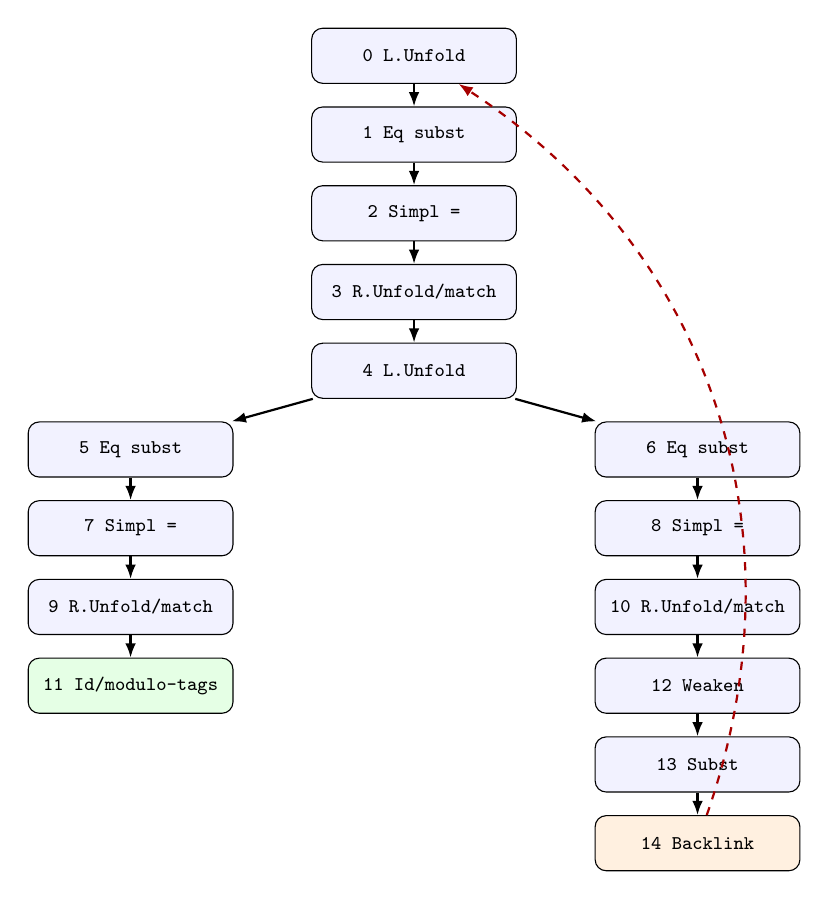
\begin{tikzpicture}[
  x=12mm,y=10mm,
  n/.style={draw,rounded corners,fill=blue!5,align=center,
            minimum width=26mm,minimum height=7mm,font=\scriptsize\ttfamily},
  a/.style={n,fill=green!10},
  b/.style={n,fill=orange!12},
  e/.style={-{Latex[length=1.8mm]},thick},
  back/.style={e,dashed,red!65!black,bend right=38}
]
\node[n] (n0) at (0,0) {0 L.Unfold};
\node[n] (n1) at (0,-1) {1 Eq subst};
\node[n] (n2) at (0,-2) {2 Simpl =};
\node[n] (n3) at (0,-3) {3 R.Unfold/match};
\node[n] (n4) at (0,-4) {4 L.Unfold};
\node[n] (n5) at (-3,-5) {5 Eq subst};
\node[n] (n6) at (3,-5) {6 Eq subst};
\node[n] (n7) at (-3,-6) {7 Simpl =};
\node[n] (n8) at (3,-6) {8 Simpl =};
\node[n] (n9) at (-3,-7) {9 R.Unfold/match};
\node[n] (n10) at (3,-7) {10 R.Unfold/match};
\node[a] (n11) at (-3,-8) {11 Id/modulo-tags};
\node[n] (n12) at (3,-8) {12 Weaken};
\node[n] (n13) at (3,-9) {13 Subst};
\node[b] (n14) at (3,-10) {14 Backlink};
\draw[e] (n0)--(n1); \draw[e] (n1)--(n2); \draw[e] (n2)--(n3);
\draw[e] (n3)--(n4); \draw[e] (n4)--(n5); \draw[e] (n4)--(n6);
\draw[e] (n5)--(n7); \draw[e] (n7)--(n9); \draw[e] (n9)--(n11);
\draw[e] (n6)--(n8); \draw[e] (n8)--(n10); \draw[e] (n10)--(n12);
\draw[e] (n12)--(n13); \draw[e] (n13)--(n14);
\draw[back] (n14) to (n0);
\end{tikzpicture}
\caption{The certified benchmark-01 graph.  The labels and targets are
reproduced by computation; the layout merely separates the base and recursive
branches.}
\label{fig:b01graph}
\end{figure}

For readability, Table~\ref{tab:b01nodes} abstracts the exact terms while
preserving the logical role of every node.
\begin{longtable}{@{}r p{0.22\textwidth}p{0.58\textwidth}@{}}
\caption{Reading the 15 nodes of the benchmark-01 graph.}
\label{tab:b01nodes}\\
\toprule
Index & Payload & Mathematical effect\\
\midrule
\endfirsthead
\toprule
Index & Payload & Mathematical effect\\
\midrule
\endhead
0 & L.Unfold & Invert tagged \(O(x)\); introduce \(E(y)\), contraction \(O(x)\), and \(x=s(y)\).  The recursive premise rank strictly decreases.\\
1 & Eq subst & Replace \(x\) by \(s(y)\) throughout the branch.\\
2 & Simpl = & Remove the resulting reflexive successor equation.\\
3 & R.Unfold/match & Match the successor clause of \(N(s(y))\), reducing the goal to \(N(y)\).\\
4 & L.Unfold & Invert \(E(y)\), producing zero and successor branches.\\
5 & Eq subst & Base branch: replace \(y\) by zero.\\
6 & Eq subst & Recursive branch: replace \(y\) by a successor.\\
7 & Simpl = & Base branch removes its reflexive equality.\\
8 & Simpl = & Recursive branch removes a reflexive constructor equality.\\
9 & R.Unfold/match & Base branch unfolds \(N(0)\) to the empty product.\\
10 & R.Unfold/match & Recursive branch unfolds the new natural-successor goal.\\
11 & Id/modulo-tags & Base branch closes because the empty RHS product is true.\\
12 & Weaken & Recursive branch drops context not required by the companion.\\
13 & Subst & Rename the remaining free variable to match the root exactly.\\
14 & Backlink & Close the recursive branch against node 0.\\
\bottomrule
\end{longtable}

The machine order and the diagram now coincide: node 11 is the base axiom,
node 12 begins recursive-branch preparation, and node 14 links to node 0.

\soundlim

The graph is accepted not because it has a backlink, but because all local
records are checked and the global witness passes.  The reproduced witness
selected tags
\[
 [0,0,0,0,0,\bot,0,\bot,0,\bot,0,\bot,0,0,0]
\]
and potentials
\[
 [0,3,2,1,0,0,6,0,5,0,4,0,3,2,1].
\]
Here \(\bot\) denotes \code{None}.  Progress is carried on left-unfold paths;
potentials bridge the intervening non-progressing edges.  The cycle closes
only after the strict semantic decrease exposed at node 0 (and again along the
recursive even branch).

\section{Cyclic proof and direct induction are the same descent seen twice}

The direct theorem descends on the hidden clause derivation height.  The cyclic
proof exposes the same descent locally on tagged left-unfold edges and lets a
finite graph represent repetition.  \code{odd_natural} packages the induction
globally in a Rocq proof term; the 15-node certificate packages it as a regular
derivation plus a trace witness.  Neither is more semantically privileged:
both ultimately rely on the ranked inversion condition of \code{models}.

The comparison is useful when extending search.  A direct lemma identifies a
mathematical invariant and supplies an independent oracle for a benchmark.
A generated graph tests whether the operational calculus, ordering, matching,
backlink preparation, and witness construction can discover that invariant.
Conflating these tests would hide exactly where automation remains incomplete.

\chapter{Limitations and precise claims}
\label{ch:limits}

\section{What is implemented soundly}

The reusable core consists of reified DNF syntax, ranked free-constructor
semantics, normalization, theorem-backed rule records, graph construction,
structural and trace checking, Boolean reflection into a semantic certificate,
and the one-way public theorem.  Identity, ex falso, propositional splitting,
the listed equality simplifiers, explicit weakening/substitution, left and
right unfolding, and exact backlinks all have local semantic and countermodel
proofs.

The strongest safe summary is:
\begin{center}
\rulebox{If \code{solvedb c J} computes to \code{true}, then the Rocq kernel can
derive \code{Cyclic.Valid J}.  Search bugs may cause missed proofs, expensive
reduction, or a rejected graph; they cannot bypass rule proofs or the
certificate soundness theorem.}
\end{center}

\section{Missing rule families}

\paragraph{Folding.}
There is no folding generator and no fold-then-backlink phase.  This is one of
the largest differences from the source prover and prevents useful companions
from being synthesized in the reverse direction of a definition.

\paragraph{General existential instantiation.}
There is no rule that tries available universal/free variables as
instantiations for an arbitrary sequent existential.  The right equation
solver is much narrower.  A new rule must be proved compatible with the
base/witness split; naïve whole-sequent substitution is not automatically
sound under the current semantics.

\paragraph{Exact multi-unification for right unfolding.}
The verified symmetric term unifier exists, but right unfolding uses
directional matching or an equation-producing fallback.  It does not reproduce
the source prover's multi-unification and residual-equation behavior.

\paragraph{Composed left/right unfolding.}
The original priority includes a composed step.  Here the two rules may occur
on consecutive nodes, but there is no dedicated composed candidate or its
search scheduling.

\section{Restricted implemented families}

\begin{itemize}[leftmargin=*]
\item Right conjunction requires fully free left and right pieces rather than
pairwise-disjoint existential sets.
\item Left equality substitution recognizes only a free variable on the left
and a free replacement.
\item Right existential solving accepts a single existential variable equated
to a free term; harder cyclic or mixed equations are rejected.
\item Right discharge requires a singleton antecedent and a free discharged
atom.
\item Left unfolding requires a singleton antecedent, a tagged selected atom,
bounded variables, and a free RHS.
\item Prepared backlink matching is directional and exact after substitution;
weakening removes only a suffix beyond a matching prefix.
\item The final backlink is exact apart from predicate tags and cannot reorder
set-like products or formulas.
\end{itemize}

Each restriction is conservative.  Removing one requires a theorem, not only a
new Boolean branch.

\section{Search and interface limitations}

Search is bounded and its fuel counts graph expansions.  \code{None} means
``not found within this scheduling and bound.''  It can result from missing
rules, restrictive side conditions, candidate order, a poor backlink, an
invalid closed graph, witness-enumeration cost, or too little fuel.  There is no
wall-clock timeout inside Gallina.

The public nine-result test includes the benchmark dispatcher.  General graph
search has reproduced benchmark 01 at fuel 16 and, according to the maintained
audit, benchmark 04 at fuel 18; these larger computations are not default-depth
coverage of the full suite.  The dispatcher should be removed only after
persisted general-search certificates cover each intended benchmark.

There is no parser for the source textual language, no definition-file loader,
no pretty-printer compatible with the CLI, no command-line proof command, no
timeout integration, and no proof-statistics interface.  Users construct
reified judgments in Gallina.

\section{Soundness is not completeness}

The implementation proves
\[
 \mathsf{success}\Rightarrow\mathsf{validity}.
\]
It does not prove
\[
 \mathsf{validity}\Rightarrow\mathsf{success},
 \qquad
 \mathsf{failure}\Rightarrow\mathsf{invalidity},
 \qquad\text{or}\qquad
 \mathsf{success}\Rightarrow\mathsf{generalDFSFoundIt}.
\]
The last implication fails specifically because a theorem-backed exact
benchmark fallback is a permitted public strategy.  This logical bookkeeping
is the most important interpretive limitation in the current system.

\chapter{Trust boundary and reproduced validation}
\label{ch:trust}

\section{What the kernel checks}

Every \code{Qed} or \code{Defined} object is checked by the Rocq kernel.  Rule
records contain proof terms; Boolean reflection lemmas are proof terms; the
certificate fields are proof terms; and the final well-founded induction is a
proof term.  Tactics such as \code{lia} and evaluation mechanisms such as
\code{vm_compute} help construct or reduce those terms but do not add unchecked
object-logic rules.  The Rocq reference manual describes this kernel-centered
trust model and the relevant commands \cite{rocq91manual}.

The trusted computing base still includes Rocq's kernel and runtime, the
standard library definitions and admitted principles explicitly reported by
\code{Print Assumptions}, the parser/elaborator used to construct terms, and the
host/compiler stack needed to run Rocq.  The LaTeX tutorial is explanatory and
not part of the proof object.

\section{Printed assumptions}

The reproduced queries at the documented revision gave:
\begin{lstlisting}[caption={Assumption audit.}]
Print Assumptions benchmark_01_valid.
(* Closed under the global context *)

Print Assumptions raw_check_sound.
(* Classical_Prop.classic *)

Print Assumptions Cyclic.certificate_sound.
(* Classical_Prop.classic *)
\end{lstlisting}
For \code{search_sound}, Rocq reported the following four standard-library
principles:
\begin{itemize}[leftmargin=*]
\item \code{FunctionalExtensionality.functional_extensionality_dep};
\item \code{ClassicalEpsilon.constructive_indefinite_description};
\item \code{Description.constructive_definite_description};
\item \code{Classical_Prop.classic}.
\end{itemize}
The direct benchmark theorem is constructive with respect to the global
context, whereas the generic cyclic route uses classical reasoning to turn a
double-negated validity argument into validity.  Search and normalization
bring in functional extensionality and choice/description principles through
their dependencies.

\soundlim

``No project-specific axioms'' is more accurate than ``axiom-free.''  The
printed output is the right evidence.  It should be rerun after changes because
refactoring definitions can alter the transitive assumption set even when a
theorem statement remains unchanged.

\section{Build and computation record}

At revision \code{08f6cd8834a3fc22088a064025abb9ee65c7f545}, before tutorial
generation, the command
\begin{lstlisting}[language=bash,numbers=none]
make -C Rocq-copy -B -j2
\end{lstlisting}
completed successfully.  It compiled the Cyclic framework, the entire
FirstOrder stack, and the other configured developments.  During that build,
assumption-printing targets reported classical logic and, for neighboring
modules, constructive definite description as expected.

The following results were independently reproduced in a Rocq 9.1.0 REPL
against the compiled tree:
\begin{itemize}[leftmargin=*]
\item the public Boolean vector is nine \code{true} values;
\item \code{certify_searched_graph 16} on normalized benchmark 01 returns a
15-node checked graph;
\item its exact node labels and target lists are those in
Chapter~\ref{ch:vertical};
\item its witness tags and potentials are those recorded there;
\item the assumption outputs are those listed above.
\end{itemize}
The project build is rerun after document generation as a regression guard.

\chapter{A theorem-first extension checklist}
\label{ch:extension}

Adding a search feature safely is easiest when the theorem boundary is fixed
before the generator.  The following sequence scales from a small simplifier
to folding or general backlink subsumption.

\begin{enumerate}[leftmargin=*]
\item \textbf{State the mathematical inference.}  Give source and premise
sequents, witness behavior, and every freshness, freeness, arity, and
occurrence side condition.
\item \textbf{Prove forward validity.}  Assume all premises valid and derive
the conclusion at an arbitrary world.  Do not mention search order.
\item \textbf{Prove countermodel propagation.}  From a false conclusion choose
an actual premise index, a target world, and a false premise.
\item \textbf{Design trace edges.}  List every valid tag pair and the subset
that strictly progresses.  Prove the non-increase and decrease inequalities.
\item \textbf{Package a \code{rule_instance}.}  Only now select the human-readable
rule name and assemble both proof fields.
\item \textbf{Write a conservative recognizer.}  Turn executable side-condition
successes into proof inputs through reflection lemmas or dependent pattern
matching.
\item \textbf{Recheck computed artifacts.}  For matching or unification, apply
the result and compare the entire structured output, not only flattened terms.
\item \textbf{Choose candidate order explicitly.}  Document interactions with
simplification, unfolding, backlinks, DFS fuel, and trace-tag selection.
\item \textbf{Add positive and negative regression equations.}  Cover success,
near misses, arity errors, variable kinds, occurs checks, and list positions.
\item \textbf{Add a checked graph regression.}  Demonstrate that a nontrivial
result reaches \code{raw_check = true}, not merely \code{graph_closedb = true}.
\item \textbf{Run the public soundness path.}  Produce a \code{verified_proof}
and derive \code{Cyclic.Valid}; never create a second unchecked result type.
\item \textbf{Audit assumptions and bounded failures.}  Run
\code{Print Assumptions}; label every \code{None} result with its exact bound
and avoid semantic conclusions from it.
\end{enumerate}

For the major missing families, the first proof obligations are already clear.
Folding needs semantic equivalence or a countermodel-directed rule plus trace
edges.  Existential instantiation needs a theorem that respects the separation
of base and witness valuations.  Full right multi-unification needs a verified
result containing a substitution and residual equations.  General backlinks
need set-level sequent subsumption and an explicit path from the current node
to an exact companion.

\appendix

\chapter{Mathematics-to-Rocq correspondence}
\label{app:correspondence}

\begin{longtable}{@{}p{0.25\textwidth}p{0.31\textwidth}p{0.35\textwidth}@{}}
\caption{Correspondence between mathematical objects and checked symbols.}\\
\toprule
Mathematical notion & Primary Rocq symbol & Important qualification\\
\midrule
\endfirsthead
\toprule
Mathematical notion & Primary Rocq symbol & Important qualification\\
\midrule
\endhead
Two variable classes & \code{var_kind}, \code{variable} & Same numeric ID may occur in each distinct kind.\\
Free term algebra & \code{term}; \code{value}; \code{eval_term} & Semantic equality is constructor-tree equality.\\
Tagged predicate atom & \code{Pred : option nat -> string -> list term -> atom} & Tag affects traces, never truth.\\
Conjunction & \code{product = list atom}; \code{product_holds} & Empty product is true.\\
DNF disjunction & \code{formula = list product}; \code{formula_holds} & Empty formula is false.\\
Sequent and environment & \code{sequent}; \code{judgment} & Judgment stores definitions with the sequent.\\
Horn production & \code{clause_body}; \code{clause_head} & Predicate name supplied by definition lookup.\\
Finite substitution & \code{substitution}; \code{subst_term} & First binding wins.\\
Right existential witness & \code{merge_valuation}; \code{right_holds} & One witness is shared by a chosen product.\\
Ranked model & \code{interpretation}; \code{models} & Introduction plus decreasing inversion.\\
Trace rank & \code{rank_atom}; \code{rank_formula}; \code{rank_of_tag} & First matching antecedent tag; missing is zero.\\
Local rule soundness & \code{rule_theorem} & Premise validity implies conclusion validity.\\
Countermodel step & \code{rule_counter_step} & Produces premise index, false world, and edge respect.\\
Non-increase/progress & \code{edge_valid}; \code{edge_progress}; \code{respects_edge} & Progress list is checked as a subset of valid pairs.\\
Finite regular proof & \code{graph}; \code{node_kind} & Backlinks target stored nodes.\\
Structural validity & \code{structural_check} & Includes reachability and absence of open nodes.\\
Size-change closure & \code{relational_trace_check}; \code{relational_check} & Required acceptance gate.\\
Finite trace routing & \code{trace_witness}; \code{witness_check} & Concrete witness used in semantic descent.\\
Proof certificate & \code{certificate}; \code{certify_raw_check} & Adds semantic evidence not decidable by generic Boolean code.\\
Infinite descent & \code{descent_measure}; \code{certificate_step_decreases} & Two-phase nested lexicographic order.\\
Semantic validity & \code{Cyclic.Valid}; \code{certificate_sound} & Universal over semantic worlds.\\
Set-style normalization & \code{normalize_judgment} & Removes duplicates but does not sort.\\
Directional match & \code{match_terms}; \code{match_terms_sound} & Pattern-to-target only; result rechecked.\\
Symmetric unification & \code{unify_terms}; \code{unify_terms_sound} & Occurs checked and fuel bounded; not fully integrated.\\
Candidate generation & \code{generate_axiom}; \code{simplification_candidate}; \code{generate_rules} & Order affects bounded discovery only.\\
Checked graph search & \code{certify_searched_graph} & Rejects invalid closed graphs and continues DFS.\\
Public decision bit & \code{solvedb} & One-way success contract only.\\
Public theorem & \code{search_sound} & Includes transitional benchmark strategies.\\
\bottomrule
\end{longtable}

\chapter{Module and symbol index}
\label{app:module-index}

\begin{longtable}{@{}p{0.25\textwidth}p{0.67\textwidth}@{}}
\caption{All documented modules and their principal symbols.}\\
\toprule
Module & Principal symbols and role\\
\midrule
\endfirsthead
\toprule
Module & Principal symbols and role\\
\midrule
\endhead
\file{FirstOrder/Syntax.v} & \code{var_kind}, \code{variable}, \code{term}, \code{atom}, \code{product}, \code{formula}, \code{sequent}, \code{clause}, \code{judgment}, exact/tag-insensitive equalities, substitutions, shifts, bounds, tags, preparation, and definition lookup.\\
\addlinespace
\file{FirstOrder/Semantics.v} & \code{value}, \code{valuation}, \code{interpretation}, \code{atom_holds}, \code{product_holds}, \code{formula_holds}, \code{merge_valuation}, \code{right_holds}, \code{models}, \code{denote}, ranks, free-fragment lemmas, and shifting lemmas; instantiates \code{Framework.Make}.\\
\addlinespace
\file{FirstOrder/Automation.v} & Duplicate normalization with semantic preservation; set-style Booleans; variable/freshness analysis; \code{match_terms}; substitution composition; occurs checking; \code{unify_terms}.\\
\addlinespace
\file{FirstOrder/Rules.v} & The semantic kernels for all axioms and rules: identity/ex-falso, propositional rules, equality rules, discharge, weakening, substitution, right/left unfolding, and backlinks; includes arbitrary-position transport.\\
\addlinespace
\file{FirstOrder/RuleGeneration.v} & Ordered scans for axioms and simplification; structural candidates; matched and standard right unfold; arbitrary-position left unfold; \code{generate_rules}; executable regressions.\\
\addlinespace
\file{FirstOrder/GraphSearch.v} & First-open expansion, exact and prepared backlinks, bounded DFS, witness heuristics/enumeration, \code{checked_graph}, certification-aware DFS, and \code{certify_searched_graph}.\\
\addlinespace
\file{FirstOrder/Certification.v} & Reflection of structure and witnesses, countermodel advance, liveness, \code{certify_raw_check}, \code{raw_check_sound}, and one-node axiom certificates.\\
\addlinespace
\file{FirstOrder/Definitions.v} & AST transcription of all 19 entries in \code{fo_definitions}, retaining source clause order.\\
\addlinespace
\file{FirstOrder/Derived.v} & Clause introduction/inversion lemmas, parity/natural rank induction, \code{P}/\code{Q} results, addition results, rank sums for \code{N2}, value depth, and the hydra proof.\\
\addlinespace
\file{FirstOrder/Benchmarks.v} & Nine positive judgments, direct validity theorems, finite benchmark index, and proof-producing exact dispatcher.\\
\addlinespace
\file{FirstOrder/Search.v} & \code{search_config}, \code{verified_proof}, normalized root transport, generated and theorem strategies, iterative deepening, \code{search}, \code{solvedb}, and \code{search_sound}.\\
\addlinespace
\file{Cyclic/Relations.v} & Two-point slope algebra, relation/path composition, bounded closure, and decreasing-diagonal checks.\\
\addlinespace
\file{Cyclic/Framework.v} & Object-logic interface, rule/axiom records, finite graph operations, structural/relation/witness checks, certificate, lexicographic measure, and \code{certificate_sound}.\\
\bottomrule
\end{longtable}

\chapter{Rule quick reference}
\label{app:rules}

This appendix collects the mathematical forms in one place.  Side conditions
are abbreviated; Chapters~\ref{ch:rules-logic}--\ref{ch:rules-cyclic} give the
semantic reason for each one.

\[
\infer[\mathrm{Id}/\tau]{A\vdash R_0\lor B\lor R_1}{B\subseteq_\tau A}
\qquad
\infer[\bot_L]{A,t\ne t,A'\vdash R}{}
\qquad
\infer[\mathsf{clash}_L]{A,c=f(\vec t),A'\vdash R}{}
\]
\[
\infer[L.\lor]{p\lor P\vdash R}{p\vdash R & P\vdash R}
\qquad
\infer[R.\land]{L\vdash a\land B}{L\vdash a & L\vdash B}
\]
\[
\infer[\mathsf{Simpl}{=}L]{A,t=t,A'\vdash R}{A,A'\vdash R}
\qquad
\infer[\mathsf{Simpl}{=}R]{L\vdash R_0\lor(B\land t=t\land B')\lor R_1}
  {L\vdash R_0\lor(B\land B')\lor R_1}
\]
\[
\infer[\mathsf{EqSubst}]{A,x=t,A'\vdash R}
  {A[x:=t],A'[x:=t]\vdash R[x:=t]}
\qquad
\infer[\exists\mathsf{Solve}]{L\vdash R_0\lor(B\land \EV_x=t\land B')\lor R_1}
  {L\vdash R_0\lor(B[\EV_x:=t]\land B'[\EV_x:=t])\lor R_1}
\]
\[
\infer[\mathsf{Discharge}_R]{a,A\vdash R_0\lor(B\land a\land B')\lor R_1}
  {a,A\vdash R_0\lor(B\land B')\lor R_1}
\]
\[
\infer[\mathsf{Inj}_L]{A,f(\vec s)=f(\vec t),A'\vdash R}
  {A,\bigwedge_i s_i=t_i,A'\vdash R}
\qquad
\infer[\mathsf{FunEq}_R]{L\vdash R_0\lor(B\land f(\vec s)=f(\vec t)\land B')\lor R_1}
  {L\vdash R_0\lor(B\land\bigwedge_i s_i=t_i\land B')\lor R_1}
\]
\[
\infer[\mathsf{Weak}]{A,E\vdash R}{A\vdash R}
\qquad
\infer[\mathsf{Subst}]{\sigma(L)\vdash\sigma(R)}{L\vdash R}
\qquad
\infer[\mathsf{Backlink}]{J}{J}
\]
\[
\infer[R.\mathsf{Unfold}/\mathsf{match}]
 {L\vdash R_0\lor(A\land P(\vec t)\land A')\lor R_1}
 {L\vdash R_0\lor(A\land\sigma(B)\land A')\lor R_1}
\quad(\sigma\vec h=\vec t)
\]
\[
\infer[R.\mathsf{Unfold}]
 {L\vdash R_0\lor(A\land P(\vec t)\land A')\lor R_1}
 {L\vdash R_0\lor(A\land B^\exists\land\vec t=\vec h^\exists\land A')\lor R_1}
\]
\[
\infer[L.\mathsf{Unfold}]
 {A,P^t(\vec u),A'\vdash R}
 {\{A,B_c^{\uparrow,t_c},\vec u=\vec h_c^\uparrow,
      P^t(\vec u),A'\vdash R\}_{c\in\mathsf{def}(P)}}.
\]

\chapter{End-to-end audit recipe}
\label{app:audit}

When evaluating a claimed proof from this development, the following compact
procedure reconstructs the entire theorem path.

\begin{enumerate}[leftmargin=*]
\item Write the exact judgment: definition environment, DNF antecedent and
succedent, variable kinds, and tags.
\item Normalize it and record which duplicate atoms/products disappear.
\item Determine whether \code{generate_axiom} succeeds.  If not, record the
first simplifier, backlink candidates, and \code{generate_rules} list in their
actual order.
\item For every installed rule inspect its \code{rule_theorem},
\code{rule_counter_step}, and edge information.  For an axiom inspect
\code{axiom_theorem}.
\item Distinguish an explicit substitution/weakening preparation node from the
final exact backlink.
\item Verify all graph nodes are reachable and closed; then separately run the
relational and finite-witness checks.
\item Record the concrete witness tags and potentials.  Identify where the
cycle makes semantic progress and where auxiliary potential bridges stay edges.
\item Follow \code{certify_raw_check}: structure supplies root, liveness, and
advance; witness reflection supplies trace transitions.
\item Apply \code{certificate_sound}, rewrite the normalized root equality,
and use normalization preservation to obtain validity of the input.
\item If the public API was used, determine whether the result came from a
generated axiom, general graph search, or an exact benchmark theorem strategy.
\item If computation returns \code{None} or \code{false}, record the exact
configuration and report only bounded non-success.
\item Run \code{Print Assumptions} on the exported theorem and preserve the
output with the result.
\end{enumerate}

For benchmark 01 this recipe yields the chain
\[
\begin{aligned}
 O(x)\vdash N(x)
 &\xrightarrow{L.\mathsf{Unfold}} \text{ranked parity premises}\\
 &\xrightarrow{\mathsf{EqSubst},\mathsf{Simpl}{=},R.\mathsf{Unfold}}
     \text{even base/recursive split}\\
 &\xrightarrow{\text{base}} \mathrm{Id}
 \qquad\text{or}\qquad
 \xrightarrow{\text{recursive}} \mathsf{Weak};\mathsf{Subst};\mathsf{Backlink}\\
 &\xrightarrow{\mathsf{raw\_check}=\mathsf{true}}
   \mathsf{certificate}
 \xrightarrow{\mathsf{certificate\_sound}}
   \Valid(O(x)\vdash N(x)).
\end{aligned}
\]

\backmatter
\chapter*{Conclusion}
\addcontentsline{toc}{chapter}{Conclusion}

The FirstOrder development turns cyclic proof search into proof-producing
automation by keeping three layers separate.  The mathematical layer gives a
free-constructor domain, shared right witnesses, and ranked inductive
definitions.  The local proof layer packages every inference with both forward
validity and countermodel propagation.  The global layer checks a finite graph,
reflects a concrete trace witness, and rules out a countermodel by lexicographic
infinite descent.

The implementation's limitations are substantial but cleanly fenced.  Folding
and general existential instantiation are missing; matching, conjunction, left
unfolding, weakening, and backlinks are restricted; fuel makes failure only
bounded non-success; and the public benchmark suite still includes exact
theorem-backed fallbacks.  There is no parser or CLI.  None of those gaps weakens
the proved success direction.  They define the agenda for theorem-first
extension: prove the semantic transformation and trace behavior, package it as
a rule record, expose it through a conservative generator, and reuse the same
checked graph-to-validity path.

\begin{thebibliography}{9}

\bibitem{brotherston2005cyclic}
James Brotherston.
\newblock Cyclic proofs for first-order logic with inductive definitions.
\newblock In Bernhard Beckert, editor, \emph{Automated Reasoning with Analytic
Tableaux and Related Methods}, volume 3702 of \emph{Lecture Notes in Computer
Science}, pages 78--92. Springer, 2005.
\newblock \href{https://doi.org/10.1007/11554554_8}%
{doi:10.1007/11554554\_8}.

\bibitem{brotherston2011sequent}
James Brotherston and Alex Simpson.
\newblock Sequent calculi for induction and infinite descent.
\newblock \emph{Journal of Logic and Computation}, 21(6):1177--1216, 2011.
\newblock \href{https://doi.org/10.1093/logcom/exq052}%
{doi:10.1093/logcom/exq052}.

\bibitem{brotherston2012generic}
James Brotherston, Nikos Gorogiannis, and Rasmus Lerchedahl Petersen.
\newblock A generic cyclic theorem prover.
\newblock In Ranjit Jhala and Atsushi Igarashi, editors, \emph{Programming
Languages and Systems: 10th Asian Symposium, APLAS 2012}, volume 7705 of
\emph{Lecture Notes in Computer Science}, pages 350--367. Springer, 2012.
\newblock \href{https://doi.org/10.1007/978-3-642-35182-2_25}%
{doi:10.1007/978-3-642-35182-2\_25}.

\bibitem{lee2001sizechange}
Chin Soon Lee, Neil D. Jones, and Amir M. Ben-Amram.
\newblock The size-change principle for program termination.
\newblock In \emph{Proceedings of the 28th ACM SIGPLAN-SIGACT Symposium on
Principles of Programming Languages}, pages 81--92. Association for Computing
Machinery, 2001.
\newblock \href{https://doi.org/10.1145/360204.360210}%
{doi:10.1145/360204.360210}.

\bibitem{rocq91manual}
The Rocq Development Team.
\newblock \emph{The Rocq Prover Reference Manual, Version 9.1}.
\newblock The Rocq Prover Project, 2026.
\newblock \url{https://rocq-prover.org/doc/v9.1/refman/index.html}.

\end{thebibliography}

\end{document}
